\documentclass{article}

\usepackage{blindtext}
\usepackage[utf8]{inputenc}

\usepackage{graphicx,fancyhdr,amsmath,amssymb,amsthm,subfig,url,hyperref}
\usepackage{algorithm}
\usepackage{algpseudocode}
\usepackage{booktabs}
\usepackage{float}
\restylefloat{table}
\usepackage[margin=1in]{geometry}
\usepackage{amsthm}
\usepackage{multirow}
\usepackage{enumitem}
%\usepackage{enumerate}
\usepackage[normalem]{ulem}
\usepackage{accents}
\usepackage{thm-restate}
\usepackage{physics}
\usepackage[numbers]{natbib}

\usepackage{todonotes}

\newcommand{\specialcell}[2][c]{%
  \begin{tabular}[#1]{@{}c@{}}#2\end{tabular}}

%----------------------- Macros and Definitions --------------------------

%%% FILL THIS OUT
\newcommand{\studentname}{Oliver Hinder}
\newcommand{\suid}{ohinder}
%%% END

\newcommand{\ubar}[1]{\underaccent{\bar}{#1}}

 
%\usepackage{algorithm,algcompatible,amssymb,amsmath}

%\renewcommand{\COMMENT}[2][.5\linewidth]{%
%  \leavevmode\hfill\makebox[#1][l]{//~#2}}
%\algnewcommand\algorithmicto{\textbf{to}}
%\algnewcommand\RETURN{\State \textbf{return} }

% If {a} then b End
\algnewcommand{\IfR}[1]{\State\algorithmicif\ #1\ \algorithmicthen}
\algnewcommand{\EndIfR}{\unskip\ \algorithmicend\ \algorithmicif}


\renewcommand{\theenumi}{\bf \Alph{enumi}}

\theoremstyle{plain}
\newtheorem{theorem}{Theorem}
\newtheorem{assumption}{Assumption}
\newtheorem{example}{Example}


\newtheorem{claim}[theorem]{Claim}
\newtheorem{observation}[theorem]{Observation}

\newtheorem{lemma}[theorem]{Lemma}
%\newtheorem{assume}[assume]{Assumption}
%\newtheorem{example}[example]{Example}


\newtheorem{corollary}[theorem]{Corollary}
\newtheorem{definition}[theorem]{Definition}
\newtheorem{remark}[theorem]{Remark}
\newtheorem{fact}[theorem]{Fact}
%\declaretheorem[name=Theorem,numberwithin=section]{thm}
%\declaretheorem[name=Lemma,numberwithin=section]{lem}


\newcommand{\matStart}{\begin{pmatrix}}
\newcommand{\matEnd}{\end{pmatrix}}

\fancypagestyle{plain}{}
\pagestyle{fancy}
\fancyhf{}
\fancyhead[RO,LE]{\sffamily\bfseries\large Stanford University}
\fancyfoot[LO,RE]{\sffamily\bfseries\large \studentname: \suid @stanford.edu}
\fancyfoot[RO,LE]{\sffamily\bfseries\thepage}
\renewcommand{\headrulewidth}{1pt}
\renewcommand{\footrulewidth}{1pt}

\graphicspath{{figures/}}


\def\CompBeta{\beta}

\def\CompBetaAgg{\sigma_{7}}

\def\ArmijoBeta{\sigma_{2}}

\def\ProxResBeta{\sigma_{3}}

\def\BetaSafeAggr{**?**}

\def\BetaSafe{\sigma_{4}}

\def\BetaBacktrack{\sigma_{5}}

\def\BetaVarTheta{\sigma_{6}}

\def\NumCon{m}
\def\NumVar{n}
\def\n{n}
\def\L{L}
\newcommand{\bigO}[1]{O\left( #1 \right)}
\newcommand{\bigSO}[1]{\hat{O}\left( #1 \right)}

\def\R{R}


\def\ResKKT{\mathcal{K}}
\def\ResPrimal{\mathcal{P}}
\def\ResComp{\mathcal{C}}
\def\MeritComp{\mathcal{\zeta}}

\def\T{\mathcal{T}_{\mu}}
\def\Q{\mathcal{Q}_{\mu}}

\def\v{v}

\def\LipP{L_{p}}
\def\LipFun{L_{0}}
\def\LipGrad{L_{1}}
\def\LipHess{L_{2}}
\def\LipCube{L_{3}}

\def\DeltaF{D_{f}}

\def\Diag{\text{Diag}}

\def\X{\mathcal{X}}

\def\Lag{\mathcal{L}}

\def\N{\mathbb{N}}


% ALGORITHMS

\def\AlgTrust{Primal-dual-trust-region}
\newcommand{\callAlgTrust}[1]{\hyperref[AlgTrust]{\Call{\AlgTrust}{#1}}}
\def\AlgMain{non-convex-IPM}
\newcommand{\callAlgMain}[1]{\hyperref[AlgMain]{\Call{\AlgMain}{#1}}}



\usepackage{enumitem}

\begin{document}

\title{A one phase IPM for non-convex optimization}
\author{Oliver Hinder, Yinyu Ye}

\algdef{SE}[SUBALG]{Indent}{EndIndent}{}{\algorithmicend\ }%
\algtext*{Indent}
\algtext*{EndIndent}

\maketitle


\newcommand{\algorithmicbreak}{\textbf{break}}
\newcommand{\obj}{f}
\newcommand{\cons}{a}
\newcommand{\nvar}{n}
\newcommand{\ncon}{m}
\newcommand{\parNumCor}{c_{\max}}
\newcommand{\parComp}{\beta_{1}}
\newcommand{\parCompAgg}{\beta_{2}}
\newcommand{\parMinStableStepSize}{\beta_{3}}
\newcommand{\parKKTReductFactor}{\beta_{4}}
\newcommand{\parObjReductFactor}{\beta_{5}}
\newcommand{\parBacktracking}{\beta_{6}}
%\newcommand{\parMinStepAgg}{\beta_{8}}
\newcommand{\parFracBoundary}{\beta_{7}}
\newcommand{\parFracBoundaryMax}{\beta_{8}}
\newcommand{\parFracBoundaryExp}{\beta_{9}}
\newcommand{\parRegularizer}{\beta_{10}}
\newcommand{\parConRegularizer}{\beta_{11}}
%\newcommand{\parFilterReduceBarrier}{\beta_{13}}
%\newcommand{\parMaxRatioPrimalMu}{\beta_{14}}

\newcommand{\parDeltaMin}{\delta_{\min}}
\newcommand{\parDeltaIncreaseFailure}{\delta_{\text{inc}}}


%\newcommand{\Filter}{\mathbb{F}}
\newcommand{\History}{\mathbb{H}}
\newcommand{\conWeight}{w}
\newcommand{\ConWeight}{W}
\newcommand{\zeroSet}{Z}
\newcommand{\nonzeroSet}{N}
\newcommand{\alphaMinAgg}{\alpha_{\min}}
\newcommand{\vioVar}{\mu}
\newcommand{\barrier}{\psi}
\newcommand{\regularizer}{r}
\renewcommand{\R}{\mathbb{R}}
\newcommand{\schur}{\mathcal{M}}
%\newcommand{\schur}[1]{\mathcal{M}#1}
\newcommand{\MatrixSchur}[2]{\mathcal{H}_{#1}(#2)}


\newcommand{\termination}{\eqref{terminate-kkt}, \eqref{terminate-primal-infeasible} or \eqref{terminate-dual-infeasible}}
\newcommand{\infeasFunc}{\Gamma}


\newcommand{\TOLinf}{\epsilon_{\textbf{inf}}}
\newcommand{\TOLmu}{\epsilon_{\textbf{mu}}}
\newcommand{\TOLopt}{\epsilon_{\textbf{opt}}}
\newcommand{\TOLunbounded}{\epsilon_{\textbf{unbd}}}
\newcommand{\maxgrad}{G}


\newcommand{\status}{\textbf{status}}
\newcommand{\success}{\textsc{success}}
\newcommand{\failure}{\textsc{failure}}

\newcommand{\feasible}{\textbf{feasible}}

\newcommand{\meritKKT}{\mathbb{K}}

\newlength\myindent % define a new length \myindent
\setlength\myindent{6em} % assign the length 2em to \myindet
\newcommand\bindent{%
  \begingroup % starts a group (to keep changes local)
  \setlength{\itemindent}{\myindent} % set itemindent (algorithmic internally uses a list) to the value of \mylength
  \addtolength{\algorithmicindent}{\myindent} % adds \mylength to the default indentation used by algorithmic
}
\newcommand\eindent{\endgroup} % closes a group

% alg
\newcommand{\simpleIPM}{Simplified-One-Phase-Non-Convex-IPM}
\newcommand{\callSimpleIPM}{\Call{Simplified-One-Phase-Non-Convex-IPM}}

\newcommand{\backtrackBlurb}{\emph{Perform a backtracking line search on the primal step $\alpha_{P}$.} Trial step sizes $\alpha_{P} \in \{\alpha^{\max}_{P}, \parBacktracking \alpha^{\max}_{P}, \parBacktracking^2 \alpha^{\max}_{P}, ... \}$ computing the trial point $(x^{+}, y^{+}, s^{+}, \mu^{+})$ as described in \eqref{eq:iterate-update}. Terminate with $\status = \success$ and return the trial point the first time all of the following conditions hold:}


\begin{abstract}
The work of \cite{wachter2000failure} suggests that infeasible start interior point methods (IPMs) developed for linear programming cannot be adapted to non-linear optimization without significant modification i.e. using a two phase or a penalty method. We propose an IPM, that by careful initialization and updates of the slack variables, is guaranteed to find an first order certificate of local infeasibility, local optimal or unboundedness. Our proposed algorithm differs from other IPM methods for non-convex programming, because we reduce primal feasibility at the same rate as the barrier parameter. This gives an algorithm with more robust convergence properties and closely resembles successful algorithms from linear programming. We implement the algorithm and compare with IPOPT subset of CUTEst problems. Our algorithm requires has a similar median number of iterations, however, fails on only 9\% compared with 16\% for IPOPT. Experiments on infeasible variants of CUTEst indicate superior performance for detecting infeasibility.

%We require less iterations on Z\% of the problems and our algorithm fails only on X\% of the problems compared with Y\% for IPOPT.
\end{abstract}

\section{Introduction}

This paper develops an interior point method for finding stationary points of the problem:
\begin{flalign}\label{original-problem} 
\min_{x \in \R^{\nvar}}{f(x)} \\
a(x) \le 0,
\end{flalign}
where the functions $a(x) : \R^{\nvar} \rightarrow \R^{\ncon}$ and $f : \R^{\nvar} \rightarrow \R$ are twice differentiable and might be non-convex. Examples of real world problems in this framework include truss design, robot control, aircraft control and aircraft design \cite[TRO11X3, ROBOT, AIRCRAFTA, AVION2]{gould2015cutest}. 

Interior point methods were first developed for linear programming \cite{karmarkar1984new}. The idea for primal-dual interior point methods originates with \cite{megiddo1989pathways}. Initially, algorithms that required a feasible starting point were studied \cite{kojima1989primal,monteiro1989interior}. However, generally one is not given an initial point that is feasible. A naive solution to this issue is to move the constraints into the objective  by adding a large penalty for constraint violation (Big-M method) \cite{mcshane1989implementation}. A more effective solution is the infeasible start algorithm of \cite{lustig1990feasibility} which has less numerical issues and a smaller iteration count than the big-M method of \cite{mcshane1989implementation}. This approach also simplified the algorithm, by avoiding the need to make a good initial guess for the size of the penalty parameters. Lustig's approach was further improved in the predictor-corrector algorithm of \cite{mehrotra1992implementation}. This algorithm reduced complementarity, duality and primal feasibility at the same rate, using an adaptive heuristic. This class of methods was shown by \cite{todd2003detecting} to converge to either optimality or infeasibility certificates (of the primal or dual). 

%This infeasible start algorithm was combined with predictor-corrector technique of Mehrotra \cite{ye1993quadratic} into an algorithm with excellent practical performance. 

This infeasible start approach of \cite{lustig1990feasibility} for linear programming naturally to non-linear optimization. 
And most interior point codes for non-convex optimization are built off these ideas \cite{vanderbei1999loqo,wachter2006implementation,byrd2006knitro}. However, \cite{wachter2000failure} showed for the problem
\begin{subequations}\label{failure-ex}
\begin{flalign}
\min { x }\\
x^2 - s_1 - 1 &= 0 \\
x - s_2 - 1/2 &= 0 \\
s_1, s_2 &\ge 0,
\end{flalign}
\end{subequations}
a large class of infeasible start algorithms fails to converge to either a local optimum or infeasibility certificate starting at any point with $x < 0$, $s_{1}, s_{2} > 0$. Following this paper, a flurry of research was published suggesting different methods for resolving this issue \cite{benson2004interior}. The main two approaches can be split into penalty methods \cite{liu2004robust, chen2006interior,curtis2012penalty,gould2015interior} and two phase algorithms \cite{wachter2006implementation}. 

Penalty methods move some measure of constraint violation into the objective. These methods require a penalty parameter $M$ that measures how much the constraint violation contributes to the objective. For large enough $M$ the algorithm will converge to an optimal solution. However, estimating this penalty parameter is difficult -- too small and the algorithm will not find a feasible solution, too big and the algorithm might be slow and suffer from numerical issues. Consequently, typically penalty methods tend to be slow \cite[Algorithm 1]{curtis2012penalty} or use complex schemes for dynamically updating the penalty parameter \cite[Algorithm 2]{curtis2012penalty}. 

The algorithm IPOPT is an example of a two phase algorithm: it has a main phase and a feasibility restoration phase  \cite{wachter2006implementation}. The main phase searches simultaneously for optimality and feasibility using a classical infeasible start method. The other phase, known as the feasibility restoration phase, aims to minimizes infeasibility. The feasibility restoration phase is only called when the main phase fails e.g. the step size is small. It is well-known that this approach has drawbacks. The algorithm has difficulties detecting infeasibility \cite[Table 15]{huang2016solution} and will fail if the feasibility restoration phase is called too close to the optimal solution. Some of these issues have been addressed by \cite{nocedal2014interior}. 

The main contribution of this paper is an infeasible start method interior point method for non-linear programming that builds on the work of \cite{lustig1990feasibility, mehrotra1992implementation} for linear programming. The algorithm avoids a big-M or a two phase approach. Furthermore, our solution to the issue in example \eqref{failure-ex} of \cite{wachter2000failure} is simple: we carefully initialize the slack variables and use non-linear updates to ensure we approach feasibility from above. Consequently, under general conditions we guarantee that our algorithm will converge to either a local certificate of optimality, local infeasibility or unboundedness. Our algorithm has other desirable properties. Complementarity moves at the same rate as primal feasibility. This implies from \cite{lagIPM} that, if certain sufficient conditions for local optimality conditions hold, our approach guarantees dual multipliers sequence will remain bounded. In contrast, methods that reduce the primal feasibility too quickly, such as IPOPT,  the dual multiplier sequence can be unbounded even for linear programs.

%From \cite{lagIPM} we know that if certain sufficient conditions for local optimality conditions hold, then a subsequence of the dual multipliers will converge if the primal solution is converging to a KKT point. Consequently, our algorithm may find finite dual multipliers, even if the set of dual multipliers at the KKT point is unbounded. Conversely, methods that reduce the primal feasibility too quickly, such as IPOPT, will suffer from divergent dual multipliers \cite{lagIPM}.

Our method has further similarities with Mehrotra's \cite{mehrotra1992implementation} predictor-corrector algorithm for linear programming: the rate that we reduce the dual feasibility, primal feasibility and complementarity is adaptive.
We implement the algorithm and compare our solver with IPOPT on large scale CUTEst problems. Our algorithm requires has a similar median number of iterations, however, seems to fail less often. Experiments on infeasible variants of CUTEst indicate superior performance for detecting infeasibility.

The paper is structured as follows: Section~\ref{sec:basic-alg} describes the algorithm, Section~\ref{sec:theory} gives the convergence proofs, Section~\ref{sec:implementation-details} delves into implementation details and Section~\ref{sec:empirical-results} presents test results on the CUTEst test set.


{\color{red}
\begin{enumerate}
\item talk about sequence stuff or MFCQ [MOVE??]
\item talk about filter methods and how people observed better performance by avoiding penalty functions (so they take bigger steps)
\end{enumerate}


Summary of contributions:

\begin{enumerate}
\item Adaptive heuristics for reduction in $\mu$
\end{enumerate}
}


%may cycle between the feasibility restoration and optimality phases. Furthermore, if the feasibility 

\section{The algorithm}\label{sec:basic-alg}


Consider a naive log barrier problems of the form:
\begin{flalign} \label{naive-log-barrier}
\min_{x \in \R^{\nvar}}{f(x) - \mu \sum_i{ \log{(-a_i(x))} } }
\end{flalign}
The idea is to solve sequence of these sub-problems with $\mu \rightarrow 0$ and $\mu \ge 0$. The log barrier transforms the non-differentiable original problem~\eqref{original-problem} into a twice differentiable log barrier function on which we can apply newton's method. However, there are issues with this naive log barrier formulation. We are rarely given a feasible starting point. Furthermore, one would like to ensure that the primal and dual variables remain bounded. To resolve these issues we consider the shifted and regularized sub-problem described as follows:
%Therefore we shift the constraints, problem and gradually reduce the
% in the primal feasibility at each iteration. This is known shifted barrier formulation is given as follows:
\begin{flalign}
\min_{x \in \R^{\nvar}} \barrier_{\mu}(x) := f(x) + \mu r(x)  - \mu  \sum_i{ \log \left( \vioVar \conWeight_i - a_i(x)  \right) } \label{shifted-barrier-problem}
\end{flalign}
With some vector $\conWeight \ge 0$ which remains fixed for all sub-problems, and some $\vioVar > 0$ which measures the size of the shift. The function $\regularizer : \R^{\nvar} \rightarrow \R$ is define by:
\begin{flalign}\label{def:regularizer}
\regularizer(x) := \parRegularizer \sum_{i = 1}^{\nvar} \sqrt{x_i^2 + 1 / \parRegularizer^2} - \parConRegularizer e^T a(x).
\end{flalign}
where $\parRegularizer, \parConRegularizer \in (0,1)$ are constants. The purpose of $\regularizer$ is to prevent the primal iterates from unnecessarily diverging. 
%\todo{say something more vague or cite theorem}
%As  $\mu \rightarrow 0$ convergent sequence of KKT solutions with $\mu \rightarrow 0$ to the shifted barrier problem \eqref{shifted-barrier-problem} will converge towards a KKT solution of the original problem.
%\todo{Comment about importance of non-linear updates and intialization}


Holistically, our technique consists of computing two types of directions: stabilization and aggressive directions. Both of these directions are computed from the same linear system with different right hand sides. Aggressive directions are equivalent to affine scaling steps \cite{mehrotra1992implementation}; since they apply a newton step directly to the KKT system, ignoring the barrier parameter $\mu$. Aggressive steps aim to simultaneously approach optimality and feasibility. However, continuously taking aggressive steps may cause the algorithm to stall or fail to converge. To remedy this we have a stabilization step. The stabilization steps keeps the primal feasibility the same i.e. uses $\eta = 0$ and aims to reduce the log barrier objective until an approximate solution to the shifted log barrier problem is found. While this step has similar goals to the centering step of Mehrotra there are distinct differences. The centering steps of Mehrotra move the iterates towards the central path, while keeping the primal and dual feasibility fixed. However, our stabilization steps only keep the primal feasibility fixed, while reducing the log barrier objective. This choice reflects challenges that occur in non-convex optimization and will be discussed more in [??]
%Section~\ref{sec:convergence-proofs}. 

The interior point method that we develop generates a sequences of primal iterates $x^{k}$, $s^{k} \in \R^{\nvar}$ with $s^k > 0$, barrier parameter $\mu^k > 0$ and feasibility violation $\vioVar^k > 0$ that satisfy:
\begin{subequations}\label{eq:barrier-primal-sequence-nice}
\begin{flalign}
a(x^{k}) + s^{k} &= \mu^k \conWeight \label{eq:primal-feasibility} \\
%\theta^{k} / \mu^{k} &= \theta^{0} / \mu^{0} \\ %\theta^{0} / \mu^{0} \text{??? maybe just write an interval here} \\
\frac{S^{k} y^{k}}{\mu^{k}} &\in [ e \parComp, e / \parComp],\label{eq:comp-slack} 
\end{flalign} 
\end{subequations}
Where $\conWeight \ge 0$ is vector selected such that at the initial point $a(x^{0}) + s^{0} = \vioVar^0 \conWeight$ and $\parComp \in (0,1)$ is an algorithmic parameter. This set of equations implies the primal feasibility and complementarity are moved at the same rate. Furthermore, there exists a subsequence of the iterates (those that satisfy the aggressive step criterion \eqref{agg-criteron}) such that: %  i.e. $x^{k} \rightarrow x^{*}$ and $s^{k} \rightarrow s^{*}$
\begin{flalign}
\frac{\| \nabla_{x} \Lag(x^{k}, y^{k}) \|_{\infty}}{\mu^k(\| y^{k} \|_{\infty} + 1)} &\le 1, \label{eq:dual-feas}
\end{flalign}
where $\Lag (x, y) := f(x) + y^T a(x)$ is the Lagragian function. Equations \eqref{eq:barrier-primal-sequence-nice} and \eqref{eq:dual-feas} holding is common in many practical linear programming implementations \cite{mehrotra1992implementation, more}. These conditions holding is desirable, because it implies the dual variables likely remained bounded. To be more precise, assume the subsequence satisfying \eqref{eq:barrier-primal-sequence-nice} and \eqref{eq:dual-feas} is converging to a feasible solution. If this solution satisfies certain sufficiency conditions for local optimality, then as shown in \cite{lagIPM} the dual variables will remain bounded. Note that \eqref{eq:barrier-primal-sequence-nice} and \eqref{eq:dual-feas} can be interpreted as a `central sequence'. This is weaker than the existence of a central path, a concept from convex optimization \cite{megiddo1989pathways,andersen1999homogeneous}. Unfortunately, in non-convex optimization there may not exist a continuous central path (see Appendix~\ref{app:non-existence-of-central-path}).

\todo{
interpretation of equality v.s. inequality constraints primal-dual methods 
}

\subsection{Derivation of direction computation}\label{sub:direction-computation}

We cannot apply a newton method directly to problem \eqref{shifted-barrier-problem} without adding a proximal term \eqref{prox-obj} parameterized by $\delta$ and centered about the previous iterate $x$. This ensures the newton direction exists and is decreasing in the objective value for a fixed constraint violation i.e. $\eta = 0$. Therefore, we find the next iterate by approximately solving:

\begin{subequations}\label{sophisticated-barrier-problem}
\begin{flalign}
x^{*}, s^{*} \gets \arg \min_{\bar{x} \in \R^{\nvar}, \bar{s} \in \R^{\ncon++}} & f(\bar{x}) -(1 - \eta) \mu \left( -\regularizer( \bar{x} ) + \sum_i{ \log{\bar{s}_i} } \right)  + \frac{\delta}{2} \| \bar{x} - x \|^2 \label{prox-obj} \\
& a(\bar{x}) + \bar{s} = (1 - \eta) \mu \conWeight \\
& \bar{s} \ge 0.
\end{flalign}
\end{subequations}

Writing the first-order local optimality conditions for this problem gives:
\begin{flalign*}
\nabla_{x} \Lag(x^{*}, y^{*}) + \delta (x^{*} - x) &=  (1 - \eta) \mu \nabla \regularizer( x^{*} )  \\
a(x^{*}) + s^{*} &= (1 - \eta) \mu \conWeight \\
s_i^{*} y_i^{*} &= (1 - \eta) \mu \\
s^{*}, y^{*} &\ge 0
\end{flalign*} 
Primal interior point methods \cite{fiacco1990nonlinear} apply Newton's method directly to system \eqref{sophisticated-barrier-problem}. However, they have inferior practical performance to primal-dual methods, that apply newton's method directly to the optimality conditions. Therefore, we use primal-dual search directions defined as follows:
\begin{flalign}\label{primal-dual-newton-direction}
\mathcal{K}_{\delta}
d
=
-b
\end{flalign}
where
\begin{flalign}
d &= \begin{bmatrix}
d_{x} \\
d_{s} \\
d_{y}
\end{bmatrix} 
\\
b &= \begin{bmatrix}
 \nabla_{x} \Lag(x,y) + (1 - \eta) \mu \nabla r(x) \\
\eta  \mu \conWeight \\
Y s - \eta \mu e 
\end{bmatrix} \label{def:b} 
\\
\mathcal{K}_{\delta}
 &= \begin{bmatrix}
 \nabla^2_{x} \Lag(x,y) + (1 - \eta) \mu \nabla^2 r(x) + \delta I  & \nabla a(x)^T & 0  \\
\nabla a(x) & 0 & I \\
0 & S & Y
\end{bmatrix}. \label{def:K-delta} 
\end{flalign}

We use $\mathcal{K}_{\delta}^{-1}$ to denote the factorization of $\mathcal{K}_{\delta}$ e.g. LDL.


By taking the primal schur complement one can see solving system \eqref{primal-dual-newton-direction} for $d_{x}$ is equivalent to solving:
%$$
%\MatrixSchur{\delta}{x,y,s,\mu}
%$$

\begin{flalign}\label{eq:schur-complement}
(\schur + \delta I)  d_{x} = - \nabla f(x) - \nabla a(x)^T ((1 - \eta) \mu S^{-1} e + \eta Y ( e +  \mu S^{-1}\conWeight ) - \mu (1 - \eta) \nabla r(x)
\end{flalign}
Where the matrix $\schur$ is
\begin{flalign}\label{eq:schur-matrix}
\schur = \nabla^2_{x} \Lag (x, y) + (1 - \eta) \mu \nabla^2 r(x)  + \nabla a(x)^T Y S^{-1} \nabla a(x),
\end{flalign}
is a primal-dual approximation of the hessian of the log barrier function $ \barrier_{\mu}(x)$. Note that if the matrix $(\schur + \delta I)$ is positive definite and $\eta = 0$ then the right hand side of \eqref{eq:schur-complement} becomes $-\nabla \barrier_{\mu}(x)$ hence the direction $d_{x}$ is a descent direction on the function $\barrier_{\mu}(x)$. Consequently, during our algorithm we will pick $\delta > 0$ such that  the matrix $(\schur + \delta I)$ is positive definite.

\todo{careful with $\nabla^2 r(x)$.}


\subsection{Updating the iterates}

Suppose that we have computed some direction $d$ by solving system \eqref{primal-dual-newton-direction}. We wish to construct a candidate $(x^{+}, s^{+}, y^{+}, \mu^{+})$ for the next iterate.
Given a primal step size $\alpha_{P}$ we update the primal iterates as follows:
\begin{subequations}\label{eq:iterate-update}
\begin{flalign}
\mu^{+} &\gets (1 - \eta \alpha_{P}) \mu \\
%\vioVar^{+} &\gets (1 - \eta \alpha_{P}) \vioVar \\
x^{+} &\gets x + \alpha_{P} d_{x} \label{eq:xVarUpdate} \\
s^{+} &\gets \vioVar^{+} \conWeight - a(x^{+}) \label{eq:slackVarUpdate}
\end{flalign}
\end{subequations}
The slack variable update \eqref{eq:slackVarUpdate} is non-linear and its purpose is to ensure that equation~\eqref{eq:primal-feasibility} remains satisfied and therefore we can control the rate of reduction of primal feasibility. However, if the function $a$ is linear the slack variable update~\eqref{eq:slackVarUpdate} reduces to:
$$
s^{+} = \vioVar^{+} \conWeight - a(x) - \alpha_{P} \nabla a(x)  d_{x} = \left(\vioVar \conWeight - a(x) \right) -  \alpha_{P}  \left( \eta \vioVar \conWeight + \nabla a(x)  d_{x} \right) = s + \alpha_{P} d_{s}
$$
Therefore if the function $a$ is linear we use the same updates as infeasible start algorithms for linear programming \cite{lustig1990feasibility,mehrotra1992implementation}. We remark that non-linear updates for the slack variables have been used in other interior point methods \cite{curtis2012penalty}.

Next, we specify a criterion to prevent the slack variables from getting too close to the boundary. In particular, given any candidate primal iterate $(x^{+}$, $s^{+})$ we require that the following fraction to the boundary rule is satisfied:
\begin{flalign}\label{fracBoundary}
s^{+} \ge  \parFracBoundary \min\{ s, \| d_{x} \|_{\infty}^2 \} 
\end{flalign}

Finally, it remains to desribe how to update the dual variables. Given some candidate primal iterate $x^{+}$, $s^{+}$, then let $B( s^{+}, d_{y} )$ be the set of feasible dual step sizes. More precisely, $B( s^{+}, d_{y} )$ is the largest interval such that if $\alpha_{D} \in B( s^{+}, d_{y} )$ then
\begin{subequations}\label{subeq:set-B}
\begin{flalign}
 \frac{S^{+} (y + \alpha_{D} d_{y})}{\mu^{+}} &\in [\parComp, 1/\parComp ] \label{satisfy-comp} %\\
% y + \alpha_{D} d_{y} &\ge  \parFracBoundary \min\{ y ,  \| d_{x} \|_{\infty}^2 \}.
\end{flalign}
\end{subequations}
If no such interval exists we set $B( s^{+}, d_{y} )$ to the empty set and the step will be rejected. We compute the dual step size as follows:
\begin{flalign}
\alpha_{D} = \arg \min_{\alpha_{D} \in B( s^{+}, d_{y} )} \| S^{+} y - \mu^{+} + \alpha_{D} S^{+} d_{y} \|^2_{2} + \| \nabla_{x} \Lag(x, y)  + (\nabla_{x}^2 \Lag(x, y) + \delta I) \alpha_{P} d_{x}  +\alpha_{D}  \nabla a(x)^T d_{y} \|^{2}_{2}.
\label{eq:alphaD-least-squares}
\end{flalign}
This reduces to a one dimensional least squares problem in $\alpha_{D}$ which has a closed form expression.

\subsection{Termination criterion}

Now, we have derived the primal infeasibility termination criterion we can present the termination criterion for our algorithm. Define the following function $\sigma$,
$$
\sigma (y) := \frac{100}{\max\{ 100, \| y \|_{\infty} \}}
$$
which is a scaling factor based on the size of the dual variables. This scaling factor is related to $s_{d}$ and $s_{c}$ in the IPOPT implementation paper \cite{wachter2006implementation}. We use $\sigma(y)$ in the local optimality termination criterion \eqref{terminate-kkt} because there may be numerical issues reducing the unscaled dual feasibility if the dual multipliers become large. In particular, the first order optimality termination criterion we use is:
\begin{subequations}\label{terminate-kkt}
\begin{flalign}
\sigma (y) \| \nabla \Lag(x, y) \|_{\infty} &\le  \TOLopt  \\
\sigma (y) \| S y \|_{\infty} &\le \TOLopt  \\
\| a(x) + s \|_{\infty} &\le \TOLopt.
\end{flalign}
\end{subequations}
The first order local primal infeasibility termination criterion is given by:
\begin{flalign}\label{terminate-primal-infeasible}
\infeasFunc (x,y,s, \vioVar) \le \TOLinf
\end{flalign}
where
\begin{flalign}\label{def:infeasFunc}
\infeasFunc (x,y,s, \vioVar) :=  \frac{\max \{ \| \nabla a(x)^T y \|_{\infty}, \| S y \|_{\infty} \}}{ \| Y\conWeight\|_{\infty} \min\{  1, \vioVar \}}.
\end{flalign}
We remark that if we find a point with $\infeasFunc (x,y,s, \vioVar) = 0$ then we if $w = e$ have found a stationary point to the problem:
\begin{flalign*}
\min_{x \in \R^{\nvar}} \max_{i \in \{1 , ..., \ncon\}}{ a_i(x) } 
\end{flalign*}
For a more thorough justification of this choice for the infeasibility termination criterion see Section~\ref{sec:infeas-criteron-justify}.

The unboundedness termination criterion is given by
\begin{flalign}\label{terminate-dual-infeasible}
\frac{\max\{ \| a(x)^{+} \|_{\infty}, 1 \}  }{\min\{ \max\{1,-f(x) \} \}, \| x \|_{\infty} \}} \le \TOLunbounded.
\end{flalign}
Satisfying this termination criterion for arbitrary small $ \TOLunbounded$ does not guarantee that the problem has an objective that is unbounded from below on the feasible region. However, if the functions $f$ and $a$ are convex, and there exists a strictly feasible solution, then if the criterion is satisfied as $\TOLunbounded \rightarrow 0$ one can conclude the objective is unbounded from below on the feasible region.

\subsection{Algorithm outline}

Before we outline our algorithm, we need to define the switching condition when take an aggressive direction instead of a stabilization step, which we define as follows:
\begin{subequations}\label{agg-criteron}
\begin{flalign}
\sigma (y) \| \nabla \Lag(x, y) \|_{\infty} &\le \mu   \label{agg-criteron-opt} \\
\| \nabla \Lag(x, y) \|_{\infty} &\le  \| \nabla f(x) \|_{\infty} + \mu / \parCompAgg \label{agg-criteron-farkas} \\
 \frac{S y}{\mu} &\in [ e \parCompAgg, e / \parCompAgg ]. \label{agg-criteron-buffer}
\end{flalign}
\end{subequations}
where the parameter $\parCompAgg \in (0, \parComp)$. The purpose of \eqref{agg-criteron-opt} is to ensure that we have approximately solved the shifted log barrier problem. Equation~\eqref{agg-criteron-farkas} also helps ensure (as we show in Section~\ref{sec:global-conv}) that if the dual variables are diverging rapidly then the infeasibility termination criterion is met. Finally, equation~\eqref{agg-criteron-buffer} with $\parCompAgg < \parComp$ ensures we have some a buffer in the complementarity such that we can still satisfy \eqref{satisfy-comp} when we move in the aggressive search direction. Algorithm~\ref{one-phase-IPM} formally outlines our one phase interior point method. Note that Algorithm~\ref{one-phase-IPM} does not include the details for the aggressive or stabilization steps that are given in Algorithm~\ref{alg:aggressive} and Algorithm~\ref{alg:stable} respectively. Since Algorithm~\ref{one-phase-IPM} maintains $a(x) + s = \conWeight \vioVar$ for each iterate, it requires the starting point satisfies:
$$
a(x^{0}) + s^{0} = \conWeight \vioVar^{0},
$$
with $\conWeight \ge 0$ and $\vioVar^{0} > 0$. For any fixed $x^{0}$ one can always pick sufficiently large $\conWeight$ and $\mu^{0}$ such that $\mu^{0} \conWeight > a(x^{0})$ and setting $s^{0} \gets \conWeight \vioVar^{0} - a(x^{0})$ meets our requirements. For the details of how initialize the variables in the practical implementation see Section~\ref{sec:initialization}.

The general idea of Algorithm~\ref{one-phase-IPM} is as follows. At each outer iteration we factorize the matrix $\mathcal{K}_{\delta}$ with an appropriate choice of $\delta$ using Algorithm~\ref{alg:mat-fact} (based off ideas of IPOPT). With this factorization fixed, we then attempt to take multiple inner iterations (at most $\parNumCor$), which corresponds solving system~\eqref{primal-dual-newton-direction} with different right hand sides choices, but the same matrix $\mathcal{K}_{\delta}$. Each inner iterations is either an aggressive or stabilization steps. If, on the inner iteration, the step fails (i.e. due to a too small step size), then we increase $\delta$ to address this failure and re-factorization $\mathcal{K}_{\delta}$. Note that we evaluate the Hessian of the Lagrangian and the full Jacobian once per outer iteration (we do one Jacobian-vector product per inner iteration).


%it is suffices to choose $\mu^{0} \conWeight > a(x^{0})$, although we choose $\conWeight_i = 1$ for

\begin{algorithm}[H]
\textbf{Input:} some initial point $x^{0}$, vector $\conWeight \ge 0$ and variables $y^{0}, s^{0}, \mu^0 > 0$  such that $a(x^{0}) + s^{0} = \conWeight \vioVar^{0}$. Termination tolerances $\TOLinf$, $\TOLunbounded, \TOLinf > 0$. \\
\textbf{Output:} some point $(x, y, s, \mu)$ that satisfies the termination criterion (inequalities \termination{}) 
\vspace{0.1 cm} \\
\emph{For each outer iteration $i \in \{1, \dots, i_{\max}\}$ perform the following steps:}
\begin{enumerate}[label*=A.{\arabic*}]
\item \label{step-1}  \emph{Evaluate the matrix Hessian of the Lagrangian $\nabla^2_{x} \Lag(x,y)$ and the Jacobian of the constraints $\nabla a(x)$.}
\item \label{line:form-K}  \emph{Form the matrices $\mathcal{K}_{0}$ and $\schur$ using \eqref{def:K-delta} and \eqref{eq:schur-matrix} respectively, at the point $(x, y, s, \mu)$ with $\eta = 1$ if the aggressive step criterion~\eqref{agg-criteron} is satisfied and $\eta = 0$ otherwise.}
%\item \emph{Form primal schur complement at the current point $\schur$ via \eqref{}.}
\item \emph{Select $\delta$ and factorize the matrix $\mathcal{K}_{\delta}$,} \\
i.e. run Algorithm~\ref{alg:mat-fact} with: \\
\hspace*{0.1cm}  \textbf{Input:} $\mathcal{K}_{0}$, $\delta$. \\
\hspace*{0.1cm} \textbf{Output:} New value for $\delta$, factorization $\mathcal{K}_{\delta}^{-1}$.
\item \label{take-steps}  \emph{Perform inner iterations.} For $j \in \{ 1, \dots , \parNumCor \}$:
\begin{enumerate}[label*=.{\arabic*}]
\item \emph{Take step}\label{line:take-step}
\begin{enumerate}[label=-Case-{\Roman*}]
\item If the aggressive step criterion~\eqref{agg-criteron} is satisfied, do an aggressive step, \\
i.e. run Algorithm~\ref{alg:aggressive} with: \\
\hspace*{0.1cm}  \textbf{Input:} $\mathcal{K}_{\delta}, \mathcal{K}_{\delta}^{-1}$ and the point $(x,y,s, \mu)$. \\
\hspace*{0.1cm}  \textbf{Output:} A $\status$ and a new point $(x^{+},y^{+},s^{+}, \mu^{+})$.
\item Otherwise, do a stabilization step, \\
i.e. run Algorithm~\ref{alg:stable} with: \\
\hspace*{0.1cm} \textbf{Input:} $\mathcal{K}_{\delta}, \mathcal{K}_{\delta}^{-1}, \schur$ and the point $(x,y,s, \mu)$. \\
\hspace*{0.1cm} \textbf{Output:} A $\status$ and a new point $(x^{+},y^{+},s^{+}, \mu^{+})$.
\end{enumerate}
\item \emph{Deal with failures}. If $\status = \success$ set $(x, y, s, \mu) \gets (x^{+},y^{+},s^{+}, \mu^{+})$. If $\status = \failure$ and $j = 1$ go to \eqref{increase-delta-for-failure}.  If $\status = \failure$ and $j > 1$ go to go to step~\eqref{step-1}.
\item \emph{Check termination criterion}. If any of the inequalities \termination{} hold at the point $(x,y,s,\mu)$ terminate the algorithm.
\end{enumerate}
\item 
Go to \eqref{step-1}.
\item \label{increase-delta-for-failure} \emph{Increase delta to address failure}. Set $\delta = \max\{\parDeltaIncreaseFailure \delta, \parDeltaMin \}$ and factorize the matrix $\mathcal{K}_{\delta}$. Go to step \eqref{take-steps}.
\end{enumerate}
\caption{High level description of one phase IPM}\label{one-phase-IPM}
\end{algorithm}

In both the aggressive steps and stabilization steps we use a backtracking line search. 
We choose the initial trial primal step size $\alpha_{P}^{\max}$ to be the maximum $\alpha_{P} \in [0,1]$ that satisfies the following fraction to the boundary rule:
\begin{flalign}\label{fracBoundaryPrimalMax}
s + \alpha_{P} d_{s} &\ge  \parFracBoundaryMax  \min\{ s, \max\{ \| d_{x} \|_{\infty}^2 , \| d_{x} \|_{\infty}^{\parFracBoundaryExp} \} \} 
\end{flalign}
where the parameter $\parFracBoundaryMax \in (\parFracBoundary, 1)$ and $\parFracBoundaryExp \in (1,2)$. The idea of this choice for $\alpha_{P}^{\max}$ is that the fraction to the boundary rule \eqref{fracBoundary} is likely to be satisfied for the first trial point i.e. $\alpha_{P} = \alpha_{P}^{\max}$. This is because:
$$
\parFracBoundaryMax  \min\{ s, \max\{ \| d_{x} \|_{\infty}^2 , \| d_{x} \|_{\infty}^{\parFracBoundaryExp} \} \} > \parFracBoundary \min\{ s, \| d_{x} \|_{\infty}^2 \} 
$$
corresponding to the right hand side of equation~\eqref{fracBoundaryPrimalMax} and equation~\eqref{fracBoundary} respectively.

\subsection{Aggressive steps}

Recall that when computing aggressive search directions we solve the system~\eqref{primal-dual-newton-direction} with $\eta = 1$, that is, we aim for both feasibility and optimality simultaneously. We accept any step size assuming it satisfies the fraction to the boundary rule \eqref{fracBoundary} and the set of valid dual step sizes are non-empty $B( s^{+}, d_{y} ) \neq \emptyset$ (see equations~\eqref{subeq:set-B}). 

The backtracking line search of the aggressive step has a minimum step size. If during the backtracking line search (line~\ref{agg:back-track} of Algorithm~\ref{alg:aggressive}) the step size $\alpha_{P}$ satisfies:
 \begin{flalign}\label{min-step-size-aggresssive}
\alpha_{P} \le \min_{i \in \{ 1, ..., \ncon \} : \conWeight_i > 0}{\frac{\parBacktracking s_{i}}{4 \vioVar \conWeight_i} } %\parMinStepAgg \times \min_{\{ j : a_j(x) + s_j < 0 \}}{ \frac{ -s_j }{ a_j(x) + s_j} },
\end{flalign}
then we immediately reject the step and exit Algorithm~\ref{alg:aggressive}. Following this, $\delta$ is increased in Line~\ref{increase-delta-for-failure} of Algorithm~\ref{one-phase-IPM} and a new aggressive step is attempted. It is possible that $\delta$ will be increased many times, however, for sufficiently large $\delta$ an acceptable step will be found (see Lemma~\ref{lemma:agg-succeeds}). 


\begin{algorithm}[H]
\textbf{Input:} The point $(x,y,s, \mu)$, the matrix $\mathcal{K}_{\delta}$ and its factorization $\mathcal{K}_{\delta}^{-1}$. \\
%Some point $p = (x, y, s, \mu)$. The matrix from the linear system~\eqref{primal-dual-newton-direction} factorized (not necessarily at the point $p$) and a corresponding inertia modification $\delta$. \\
\textbf{Output:} A new point $(x^{+}, y^{+}, s^{+}, \mu^{+})$ and a $\status$ of either $\success$ or $\failure$
\begin{enumerate}[label*=A.{\arabic*}]
\item Compute the vector $b$ at the point $(x,y,s, \mu)$ via \eqref{def:b} with $\eta = 1$.
\item Solve the system $\mathcal{K}_{\delta} d = -b$.
\item Estimate the largest primal step size $\alpha^{\max}_{P}$ from equation~\eqref{fracBoundaryPrimalMax}.
\item \label{agg:back-track} \backtrackBlurb
\begin{enumerate}[label=({\roman*})] 
\item The fraction to the boundary rule \eqref{fracBoundary} is satisfied
\item The set of valid dual step sizes is non-empty i.e. $B( s^{+}, d_{y} ) \neq \emptyset$ 
%\item If either fraction to the boundary rule \eqref{} is satisfied or $\meritKKT_{\mu} ( x^{+}, y^{+}, s^{+} )  \le \beta (\| a(x^{+}) + s^{+} \|_{\infty} + \| a(x^{+}) + s^{+} \|_{\infty}^{1/2}) $
\end{enumerate}
Terminate with $\status = \failure$ if the line search step size with \eqref{min-step-size-aggresssive} satisfied.
\end{enumerate}
\caption{High level description of aggressive step}\label{alg:aggressive}
\end{algorithm}


\subsection{Stabilization step}

\subsubsection{Augmented log barrier merit function}\label{sec:augmented-log-barrier}

When the stabilization step is called the goal is to minimize the function $\barrier_{\mu}$ keeping the constraint violation and barrier parameter fixed, until criterion~\eqref{agg-criteron} for an aggressive step is met. For this reason, it makes sense to use the log barrier function $\barrier_{\mu}$ to measure progress. We can approximate the change in the log barrier function by the following model:
\begin{flalign}
\tilde{\Delta}_{(x,y)}^{\barrier_{\mu}} ( u ) = \frac{1}{2} u^T \schur u + \nabla \barrier_{\mu}(x)^T u
\end{flalign}
where $\schur$ is computed on line~\ref{line:form-K} of Algorithm~\ref{one-phase-IPM}.

Note that if $\schur = \nabla^2_{\mu} \barrier(x)$ then $\tilde{\Delta}_{(x,y)}^{\barrier}$ becomes the second order taylor approximation of $\barrier_{\mu}$ at the point $x$. Thus, we can think of $\tilde{\Delta}_{(x,y)}^{\barrier} ( u )$ as a primal-dual approximation of the barrier function $\barrier_{\mu}$. Note that the log barrier function  does not measure anything with respect to the dual iterates. This might impede performance if $\| S y - \mu \|_{\infty}$ is large, but $\| \nabla \barrier_{\mu}(x) \|$ is small. In this case, taking a large step might reduce the complementarity significantly, even though the barrier function increases slightly. Therefore we add a complementarity measure to the barrier function to create an augmented log barrier function:
\begin{flalign}
\phi_{\mu}(x, y, s) := \barrier_{\mu}(x) + \MeritComp(s, y),
\end{flalign}
where
$$
\MeritComp(s,y) = \frac{\| S y - \mu \|_{\infty}^3}{\mu^2}.
$$
We can also build a model of the $\MeritComp(s,y) $ as follows:
\begin{flalign*}
\tilde{\Delta}^{\MeritComp}_{(x,y)}( u, v ) = \frac{\| S y + Y \nabla a(x) u + S v - \mu e \|_{\infty}^3 - \| S y - \mu  \|_{\infty}^3}{\mu^2}
\end{flalign*}
and our model of $\phi_{\mu}$ is
\begin{flalign}
\tilde{\Delta}^{\phi_{\mu}}_{(x,y)}(u, v) = \tilde{\Delta}^{\barrier_{\mu}}_{(x,y)}( u ) +   \tilde{\Delta}^{\MeritComp}_{(x,y)}( u, v ).
\end{flalign}



We say that the candidate iterates $x^{+}, y^{+}, s^{+}$ have made sufficient progress on $\phi$ over the current iterate $x, y, s$ if:
\begin{flalign}\label{phi-sufficient-progress}
\phi_{\mu}(x^{+}, y^{+}, s^{+}) \le \phi_{\mu}(x, y, s) + \parObjReductFactor \tilde{\Delta}^{\phi_{\mu}}_{(x,y)}(\alpha_{P} d_{x}, \alpha_{P} d_{y})
\end{flalign}
where $\parObjReductFactor \in (0,1)$ is a user defined parameter. 

\subsubsection{KKT merit function and filter}

In the stabilization search directions we accept steps that make progress one on of two merit functions, which form a filter. The first function $\phi_{\mu}$ is defined in Section~\ref{sec:augmented-log-barrier}. The second function, we call the KKT merit function, measures the scaled dual feasibility and complementary:
\begin{flalign}\label{merit-KKT}
\meritKKT_{\mu} ( x, y, s )  = \sigma( y ) \max\{ \| \nabla \Lag(x, y ) \|_{\infty},  \| S y - \mu \|_{\infty} \}
\end{flalign}
This merit function measures progress effectively in regimes where the matrix $\schur$ is positive definite. In this case, the search directions generated by \eqref{eq:schur-complement} will be a descent direction on this merit function\footnote{For inner iteration $j=1$}. This merit function is similar to the types of the potential functions used in interior point methods for convex optimization \cite{andersen1998computational,huang2016solution}. Unfortunately, while this merit function may be an excellent choice for convex problems, in non-convex optimization it has serious issues. In particular, the search direction \eqref{eq:schur-complement} will not be a descent direction on this merit function. Moreover, changing the search direction to minimize the dual feasibility has negative ramifications. The algorithm could to converge to a critical point of the dual feasibility where $\meritKKT_{\mu} ( x, y, s ) \neq 0$\footnote{To see why this occurs one need only consider an unconstrained problem e.g. minimizing the function $f(x) = x^4 + x^3 + x$ subject to no constraints. The point $x = 0$ is a stationary point for the gradient of $\nabla f(x)$, but is not a critical point of the function.}. For further discussion of these issues see \cite{shanno2000interior}.
%\cite{shanno1997interior}.


While it is sufficient to guarantee convergence by accepting steps if \eqref{phi-sufficient-progress} is satisfied, in some regimes e.g. when $\schur$ is positive definite, this may select step sizes $\alpha_{P}$ that are too conservative.  For example, this naturally occurs near points satisfying the sufficient conditions for local optimality. In these situation often the KKT error is a better measure of progress towards a local optimum than a merit function that discards information about the dual feasibility. Furthermore, from our experience, when converging towards an optimal solution numerical errors in the function $\phi_{\mu}$ may cause the algorithm to fail to make sufficient progress on the merit function $\phi_{\mu}$ i.e. \eqref{phi-sufficient-progress} is not satisfied for any $\alpha_{P}$. For these reasons we decide to use a filter approach \cite{fletcher2002nonlinear,wachter2006implementation}. Typical filter methods \cite{fletcher2002nonlinear} require progress on either the constraint violation or objective function. Our approach is distinctly different, because we accept steps that make progress on either the merit function $\phi_{\mu}$ or the merit function $\meritKKT_{\mu}$.
% where we accept any step that makes sufficient progress on the function $\phi$ i.e. \eqref{phi-sufficient-progress}  or sufficient progress is made on the KKT merit function relative to historical iterates. 
To be precise we accept any iterate $(x^{+}, y^{+}, s^{+}, \mu^{+})$ that makes sufficient progress on the augment log barrier function $\phi_{\mu}$, or satisfies the following two equations
\begin{subequations}\label{eq:filter}
\begin{flalign}
\meritKKT_{\mu} (x^{+}, y^{+}, s^{+}) &\le (1 - \parKKTReductFactor \alpha_{P} ) \meritKKT_{\mu} (\hat{x}, \hat{y}, \hat{s}) \label{eq:kkt-progress} \\
\phi_{\mu}(x^{+}, y^{+}, s^{+}) &\le \phi_{\mu}(\hat{x}, \hat{y}, \hat{s}) + \sqrt{\meritKKT_{\mu} (\hat{x}, \hat{y}, \hat{s})} % + \meritKKT_{\mu} (\hat{x}, \hat{y}, \hat{s})^2 \right), \alpha_{P}
\end{flalign} %\parFilterReduceBarrier
\end{subequations}
 for every previous iterate $(\hat{x}, \hat{y}, \hat{s}, \hat{\vioVar})$ with $a(\hat{x}) + \hat{s} = a(x) + s$.

The idea of \eqref{eq:filter} is that for points with similar values on the augmented log barrier function the KKT error is a good measure of progress. However, we want to discourage the algorithm from significantly increasing the augmented log barrier function while reducing the KKT error. Since, if this is occurring the algorithm might converge to a saddle point. 



\subsubsection{Stabilization step algorithm}

During the backtracking line search we terminate with $\status = \failure$ if:
\begin{flalign}\label{eq:min-step-size-stable}
\alpha_{P} \le \parMinStableStepSize.
\end{flalign}
When this occurs we exit Algorithm~\ref{alg:stable} and go to line~\ref{increase-delta-for-failure} of Algorithm~\ref{one-phase-IPM}. On line~\ref{increase-delta-for-failure} we increases the size of $\delta$ and a new stabilization step is attempted. From Lemma~\ref{lem:stbl-success} we know for sufficiently large $\delta$ the stabilization step will succeed.

To ensure that we do not perform unnecessary line searches we only attempt a stabilization line search if the following inequalities holds:
\begin{flalign}
\tilde{\Delta}^{\phi_{\mu}}_{(x,y)}(d_{x}, d_{y}) < 0 \label{eq:obj-could-improve}
\end{flalign}
The idea of this equation is to only take steps when it is possible that $\phi$ can be decreased.
%\delta \| d_{x} \|_{\infty} &\le (1 - \parKKTReductFactor) \max\{ \| \nabla \Lag(x, y ) \|_{\infty}, \| S y - \mu \|_{\infty} \} \label{eq:KKT-could-improve} \\


\begin{algorithm}[H]
\textbf{Input:} The point $(x,y,s, \mu)$, the matrix $\mathcal{K}_{\delta}$ and its factorization $\mathcal{K}_{\delta}^{-1}$. \\ An approximate log barrier hessian $\schur$. \\
\textbf{Output:} A new point $(x^{+}, y^{+}, s^{+}, \mu^{+})$ and a $\status$ of either $\success$ or $\failure$
\begin{enumerate}[label*=A.{\arabic*}]
\item Compute the vector $b$ at the point $(x,y,s, \mu)$ via \eqref{def:b} with $\eta = 0$.
\item Solve the system $\mathcal{K}_{\delta} d = -b$.
\item \emph{Check that the direction has a reasonable chance of being accepted.} If \eqref{eq:obj-could-improve} is not satisfied then terminate with $\status = \failure$.
\item Estimate the largest primal step size $\alpha^{\max}_{P}$ from equation~\eqref{fracBoundaryPrimalMax}.
\item \backtrackBlurb \label{line:sbl-backtrack}
\begin{enumerate}[label=({\roman*})] 
\item The fraction to the boundary rule \eqref{fracBoundary} is satisfied.
\item The set of valid dual step sizes is non-empty i.e. $B( s^{+}, d_{y} ) \neq \emptyset$.
\item \emph{Sufficient progress on filter.} Either equation~\eqref{phi-sufficient-progress} or \eqref{eq:filter} is satisfied.
\end{enumerate}
Terminate with $\status = \failure$ if the step size becomes too small i.e. equation~\eqref{eq:min-step-size-stable} is satisfied.
\end{enumerate}
\caption{High level description of stabilization steps}\label{alg:stable}
\end{algorithm}






\subsection{Algorithm Parameters}

\begin{table}[H]
\begin{tabular}{ |c| p{7cm}|c|c| } 
 \hline
Parameter & Description & Possible values & Chosen value  \\ 
 \hline
$\parNumCor$ & Maximum number of steps per outer iteration. See \eqref{take-steps} of Algorithm~\ref{one-phase-IPM}.  & Any natural number & $3$  \\ 
 \hline
  $\parComp$ & Restricts how far complementarity of $s$ and $y$ can be from $\mu$. See \eqref{satisfy-comp}.  & The interval $(0,1)$ & $0.01$ \\ 
 \hline
   $\parCompAgg$ & Restricts how far complementarity of $s$ and $y$ can be from $\mu$ in order for the aggressive criterion to be met. See \eqref{agg-criteron-buffer}.  & The interval  $(0, \parComp)$ & $0.02$  \\ 
    \hline
   $\parMinStableStepSize$ & Minimum step size for stable line searches. See \eqref{eq:min-step-size-stable}.  & The interval $(0,1)$ & $2^{-5}$  \\ 
   \hline 
      $\parKKTReductFactor$ & Acceptable reduction factor for the scaled KKT error $\meritKKT_{\mu}$ during stabilization steps. See \eqref{eq:kkt-progress}.  & The interval $(0,1)$ & 0.2 \\ 
      \hline
            $\parObjReductFactor$ & Acceptable reduction factor for the merit function $\phi_{\mu}$ during stabilization steps. See \eqref{phi-sufficient-progress}.  & The interval $(0,1)$ & 0.1  \\
    \hline
    $\parBacktracking$ & Backtracking factor for line searches in Algorithm~\ref{alg:aggressive} and \ref{alg:stable}. & The interval $(0,1)$ & 0.5 \\
\hline
 $\parFracBoundary$ & Fraction to the boundary parameter.  & The interval $(0,1)$ & 0.01 \\ 
        \hline
$\parFracBoundaryMax$ & Fraction to the boundary parameter used in \eqref{fracBoundaryPrimalMax} for computing the maximum step size $\alpha_{P}^{\max}$. & The interval $(\parFracBoundary,1)$ & $0.2$ \\
\hline
$\parFracBoundaryExp$ & Exponent of $\| d_{x} \|$ used in fraction to boundary formula \eqref{fracBoundaryPrimalMax} for computing the maximum step size $\alpha_{P}^{\max}$. & The interval $(1,2)$ & 1.5 \\
\hline
$\parRegularizer$ & Used in the regularizer defined in \eqref{def:regularizer}. & The interval $(0,\infty)$ & $10^{-8}$ \\
\hline
$\parConRegularizer$ & Used in the regularizer defined in \eqref{def:regularizer}. & The interval $(0,\infty)$ & $10^{-4}$ \\
\hline
$\parDeltaMin$ & & The interval $(0,\infty)$ & $10^{-8}$ \\
\hline
$\parDeltaIncreaseFailure$ & &The interval $(1,\infty)$ & $8$ \\
\hline
\end{tabular}
\caption{Parameters values and descriptions}
\end{table}


\section{Theoretical justification}\label{sec:theory}

The goal of this Section provide some simple theoretical justification for our algorithm. Section~\ref{sec:infeas-criteron-justify} justifies infeasibility termination criterion. Section~\ref{sec:theory-naive} provides a simplified version of our algorithm, this is used to explain our algorithms global convergence properties. Section~\ref{sec:global-conv} proves that the algorithm described in Section~\ref{sec:basic-alg} eventually converges. 

\subsection{Derivation of primal infeasibility termination criterion} \label{sec:infeas-criteron-justify}

The purpose of this section is to justify our choice of local infeasibility termination criterion, by showing that it corresponds to stationary measure for the infeasibility with respect to a weighted $L_{\infty}$ norm. We also prove when the problem is convex our criterion certifies global infeasibility.

Consider the following optimization problem:
\begin{subequations}\label{infeasible-problem}
\begin{flalign}
\min_{x} \max_i{ \bar{w}_i a_i(x) }  \\
\text{s.t. } a_i(x) \le 0, \forall i \in \zeroSet
\end{flalign}
\end{subequations}

For some non-negative vector $\bar{w}$ with  $\bar{w}_i = 0$ if and only if $i \in \zeroSet$. For example, a natural choice $\zeroSet$ is the indices of constraints that have been chosen to be satisfied throughout the algorithm i.e. the bound constraints and $\bar{w}_i = 1$ for $i \not\in \zeroSet$. In this case, the problem reduces to
\begin{flalign*}
\min_{x} \max_i{ a_i(x) }  \\
\text{s.t. } a_i(x) \le 0, \forall i \in \zeroSet
\end{flalign*}
Note that \eqref{infeasible-problem} is equivalent to the following optimization problem:
\begin{subequations}\label{feas-problem}
\begin{flalign}
\min \vioVar \\
\text{s.t. } a(x) + s = \vioVar \conWeight \\
s, \vioVar \ge 0,
\end{flalign}
\end{subequations}
where the vector $w$ is defined by $w_i = \bar{w}_i^{-1}$ for $i \not\in \zeroSet$ and $w_i = 0$ for $i \in \zeroSet$. 

The KKT conditions for this problem are:
\begin{flalign*}
a(x) + s = \vioVar \conWeight  \\
\nabla a(x)^T \tilde{y}  = 0 \\
\conWeight^T \tilde{y}  + u = 1 \\
u \vioVar = 0  \\
\tilde{y}^T s = 0 \\
u, \vioVar \ge 0.
\end{flalign*}
Note that if the point $x,y,s, \vioVar$ satisfies:
\begin{flalign*}
a(x) + s = \vioVar \conWeight  \\
\infeasFunc (x,y,s, \vioVar) = 0 \\
\vioVar > 0
\end{flalign*}
then we have found an stationary point problem~\eqref{infeasible-problem} with $\vioVar > 0$. In other words, a first order infeasibility certificate. 

In the case, of convexity a stronger statement can be made:

\begin{lemma}
Assume the constraint function $a$ is convex and that some minimizer $(x^{*}, \mu^{*})$ of \eqref{feas-problem} satisfies $\| x - x^{*} \|_{2} \le R$ for some constant $R > 0$. Suppose also that at some point $(x,y,s,\mu)$ one has:
\begin{flalign}
a(x) + s &= \vioVar \conWeight \label{eq:assume-primal-good} \\
\infeasFunc (x,y,s, \vioVar) &\le \frac{1}{2 m ( R + 1)}. \label{eq:assume-infeas-criteron-holds}
\end{flalign}
Then the system $a(x) \le 0$ has no feasible solution.
\end{lemma}
\begin{proof}
Using $\tilde{y} := \frac{y}{\| Y\conWeight\|_{\infty}}$ we can write:
\begin{flalign*}
\tilde{y}^T a(x^{*}) &\ge \tilde{y}^T a(x) + \tilde{y}^T \nabla a (x) (x^{*} - x) \\
&= \tilde{y}^T (w \mu - s) + \tilde{y}^T \nabla a (x) (x^{*} - x) \\
&\ge \mu - m (1 + R) \infeasFunc (x,y,s, \vioVar) \min\{  1, \vioVar  \} \\
&> \mu/2
\end{flalign*}
The first transition holds via convexity, the second by \eqref{eq:assume-primal-good}, the third by the definition of $\infeasFunc$ and the final inequality by \eqref{eq:assume-infeas-criteron-holds}. Therefore there exists no feasible solution to $a(x) \le 0$. This is a typical Farkas infeasibility certificate argument.
\end{proof}

\subsection{Global convergence proofs for a naive algorithm}\label{sec:theory-naive}

Here we present Algorithm~\ref{alg:naive}, a naive version of Algorithm~\ref{one-phase-IPM}. The goal of this naive algorithm is to illustrate the ideas of the global convergence proof of Algorithm~\ref{one-phase-IPM}. One should think of Algorithm~\ref{alg:naive} as mimicking the worst case performance of Algorithm~\ref{one-phase-IPM}. However, in practice, Algorithm~\ref{alg:naive} would be much slower than  Algorithm~\ref{one-phase-IPM}. We emphasize that the goal of these convergence proofs is to prove asymptotic convergence to a stationary point, not to give a fast theoretical runtime bound. For work on fast theoretical runtimes for interior point methods with non-convex constraints see [REF OUR PAPER]. 
%\cite{ye1998complexity, bian2015complexity}

\begin{algorithm}[H]
\textbf{Input:} Some point $x^{0}$ and $\mu^{0} > 0$ with $a(x^{0}) < \mu^{0} e$ \\

For $k = 0, ..., \infty$
\begin{enumerate}[label*=A.{\arabic*}]
\item \label{stabilization-stage} \emph{Stabilization stage}. Starting from $x^{k-1}$ find any stationary point to the shifted log barrier problem $\min_{x} \barrier_{\mu^{k}}(x)$ i.e.
$$
x^{k} \in \{ x \in \R^{n} : \nabla \barrier_{\mu^{k}}(x) = 0 \}
$$
%$\barrier_{\mu}(x^{k+1}) \le \barrier_{\mu}(x^{k})$
%starting from the point $x^{k-1}$ find a stationary point $x^{k}$, or show the problem is unbounded from bellow i.e. generate a sequence $\hat{x}^{i}$ such that $\barrier_{\mu^k,\mu^k}(\hat{x}^{i}) \rightarrow -\infty$.
\item \emph{Update dual and slack variables}. Set 
\begin{subequations}
\begin{flalign}
s^{k} &\gets \mu^{k} e - a(x^{k}) \label{naive:stb:s} \\
y^{k} &\gets \mu^{k} (S^{k})^{-1} e. \label{naive:stb:y}
\end{flalign}
\end{subequations}

\item \emph{Check termination criterion}. If \termination{} is satisfied then terminate the algorithm.
\item \label{agg-stage} \emph{Aggressive stage}. Set
\begin{subequations}
\begin{flalign}
\alpha^k_{P} &\gets \frac{1}{2} \min\left\{ 1, \frac{\min_i\{ s_i^{k} \}}{\mu^k} \right\} \label{naive:agg:alpha} \\
\mu^{k+1} &\gets \mu^{k} (1 - \alpha^k_{P} )  \label{naive:agg:mu} \\
\bar{s}^{k} &\gets \mu^{k+1} - a(x^{k})  \label{naive:agg:s} \\
\bar{y}^{k} &\gets (\bar{S}^{k})^{-1} \bar{\mu}^{k}. \label{naive:agg:y}
\end{flalign}
\end{subequations}
\end{enumerate}
\caption{Naive version of Algorithm~\ref{one-phase-IPM}}\label{alg:naive}
\end{algorithm}

We now describe the similarities between Algorithm~\ref{one-phase-IPM} and Algorithm~\ref{alg:naive}. First note that the sequence:
\begin{flalign}
(x^{k}, s^{k}, y^{k}, \mu^{k})
\end{flalign}
corresponds to the subsequence satisfying the aggressive step criterion \eqref{agg-criteron} in Algorithm~\ref{one-phase-IPM}. Furthermore, the sequence
\begin{flalign}\label{eq:worst-case-agg-sequence}
(x^{k}, \bar{s}^{k}, \bar{y}^{k}, \mu^{k+1})
\end{flalign}
corresponding to the subsequence of iterates generated by Algorithm~\ref{alg:aggressive} i.e. aggressive steps.

Now, we can describe the similarities between Algorithm~\ref{one-phase-IPM} and Algorithm~\ref{alg:naive}. In Algorithm~\ref{one-phase-IPM}, the stabilization step is repeatedly called until the aggressive step criterion~\eqref{agg-criteron} is met. This series of consecutive stabilization steps can be viewed as equivalent one call to the stabilization stage in Algorithm~\ref{alg:naive}. Now, during an aggressive steps in Algorithm~\ref{one-phase-IPM}, if we let $\delta \rightarrow \infty$ then $x^{+} \rightarrow x$. Hence \eqref{eq:worst-case-agg-sequence} can be thought of as the `worst case' aggressive sequence, corresponding to huge choice of $\delta$. Now,
% the primal variable updates \eqref{eq:xVarUpdate} and \eqref{eq:slackVarUpdate} reduce to $s^{+} \gets s - \alpha_{P} e$ and $x^{+} \gets x$ which is roughly equivalent to the aggressive stage of Algorithm~\ref{alg:naive} since:
\begin{flalign}
\bar{s}^{k} = \mu^{k+1} e - a(x^{k}) = \mu^{k+1} e - (\mu^{k} e - s^{k} )  = s^{k} - \mu^{k} \alpha^k_{P} \ge s^k / 2 > 0%\label{eq:bar-s-k}
\end{flalign}
where the first equality follows by \eqref{naive:agg:s}, second by \eqref{naive:stb:s}, the third by \eqref{naive:agg:mu}, and the first inequality from \eqref{naive:agg:alpha}. Hence each point $x^{k}$ satisfies $\mu^{k+1} e - a(x^{k}) > 0$ and is therefore a strictly feasible starting point to the shifted log barrier problem 
$\barrier_{\mu^{k+1}}(x)$ defined in line~\ref{stabilization-stage} of Algorithm~\ref{alg:naive}. 

For simplicity of exposition, in Algorithm~\ref{alg:naive}, we assume that we have some oracle that will find a stationary point of the sub-problem $\min_{x} \barrier_{\mu^k}(x)$ given an initial point $x^{k}$. Most descent algorithms for unconstrained optimization will achieve this, assuming $f$ and $a$ are continuously differentiable. We show the convergence of the stabilization steps for this solving these sub-problems in Section~\ref{sec:global-conv}. 

In Theorem~\ref{thm:naive} we show this naive algorithm (Algorithm~\ref{alg:naive}) eventually terminates. Here we sketch the proof. Assume, that at each $x^{k}$ the first order local infeasibility is not satisfied (since otherwise the algorithm trivially terminates). A consequence of this assumption is that the dual variables are bounded from above. Since the dual variables are bounded above, we can bound the slack variables away from zero. By applying the update formula for $\mu^{k}$ given in \eqref{naive:agg:mu} we conclude $\mu^{k}$ is reduced sufficiently at each iteration and therefore $\mu^{k} \rightarrow 0$. Finally, observe that the iterates of Algorithm~\ref{alg:naive} satisfy
\begin{subequations}
\begin{flalign}
a(x^{k}) + s^{k} &= e \mu^k \\
\nabla \Lag(x^{k}, y^{k}) &= 0 \\
S^{k} y^{k} &= \mu^k e \\
s^{k}, y^{k} &\ge 0
\end{flalign}
\end{subequations}
which is the central sequence property defined in equations \eqref{eq:barrier-primal-sequence-nice} and \eqref{eq:dual-feas}, with $\conWeight = e$, as we discussed in the introduction. Hence, since $\mu^k \rightarrow 0$ eventually the optimality criterion is satisfied.


\begin{theorem}\label{thm:naive}
Assume that: 
\begin{enumerate}
\item The functions $f : \R^{\nvar} \rightarrow \R$ and $a : \R^{\nvar} \rightarrow \R^{\ncon}$ are differentiable on $\R^{\nvar}$.
\item The input parameters satisfy $\TOLopt \in (0, 1)$. %, \TOLinf, \TOLunbounded
\item The level sets of the function $\barrier_{\mu}(x)$ are bounded for all $\mu \le \mu^{0}$.
\item There exists some $\maxgrad \ge \max\{ \mu^{0}, \TOLinf \}$ such that $\| \nabla f(x^k) \|_{\infty} \le \maxgrad$.
\end{enumerate}
Then at any iteration $k$ where the infeasibility termination criterion~\eqref{terminate-primal-infeasible} is not satisfied,
$$
\| y^{k} \|_{\infty} \le \frac{2 G}{ \TOLinf \TOLopt}.
$$
Furthermore, Algorithm~\ref{alg:naive} terminates in at most 
$$
1 + \frac{4 \maxgrad}{\TOLopt \TOLinf } \log\left( \frac{\mu^{0}}{\TOLopt} \right)
$$
iterations.
\end{theorem}

\begin{proof}
First observe by the assumption that the level sets of $\barrier_{\mu^k}(x)$ are bounded and the existence of a feasible solution $x^{k}$, the set $ \{ x \in \R^{n} : \nabla \barrier_{\mu^{k}}(x) = 0 \}$ is non-empty (since it contains $\arg \min_{x} \barrier_{\mu^{k}}(x)$ ). Next, we have
\begin{flalign*}
\| y^{k} \|_{\infty} &\le \frac{\| \nabla a(x^k)^T y^k \|_{\infty} + \| Y^k s^k \|_{\infty}}{ \TOLinf \min\{  1, \mu^k \}} \\
& \le  \frac{\| \nabla f(x^{k}) \|_{\infty} + \mu^{k}}{ \TOLinf \min\{  1, \mu^{k} \}} \\
& \le \frac{2 G}{ \TOLinf \TOLopt} 
\end{flalign*}
where the first inequality follows from the fact that the \eqref{terminate-primal-infeasible} is not satisfied; the second inequality from $\| \nabla \Lag (x^k , y^k) \|_{\infty} = 0$ and $S^k y^k = \mu^k$. The third from $G \ge \mu^{k}$ and $\TOLopt \le 1$.
Now,
\begin{flalign*}
\mu^{k+1} &\le \mu^k  - (1/2) \min_{i}{s_{i}^{k} } \\
&= \mu^k \left( 1 - \frac{1}{2 \| y^{k} \|_{\infty}} \right) \\
&\le \mu^{k} \left(1 - \frac{\TOLopt \TOLinf }{4 \maxgrad} \right)
\end{flalign*}
where the second equality holds from $S^k y^{k} = \mu^k e$, the second inequality by our bound on $\| y^k \|_{\infty}$.
Noting that $\mu^k \le \TOLopt$ implies the algorithm terminates, gives the result. 
\end{proof}

Keep in mind that Theorem~\ref{thm:naive} only bounds the number of iterations and excludes the computational cost of each solve of the stabilization stage.

\subsection{Global convergence proofs for Algorithm~\ref{one-phase-IPM}}\label{sec:global-conv}

The majority of this section will be in the appendix for the real paper. The main result is Theorem~\ref{thm:global-convergence} which shows global convergence of Algorithm~\ref{one-phase-IPM} to a point satisfying the termination criterion.

\subsubsection{Convergence of aggressive steps}

The goal of this section is show that after a finite number of calls to aggressive steps Algorithm~\ref{one-phase-IPM} converges.
Lemma~\ref{lem:agg-finite} does not rule out the possibility of an infinite sequence of failing aggressive steps.  

\begin{lemma}\label{lem:agg-finite}
Assume that:
\begin{enumerate}
\item The functions $f : \R^{\nvar} \rightarrow \R$ and $a : \R^{\nvar} \rightarrow \R^{\ncon}$ are twice differentiable. 
\item There exists some constant $G \ge \mu^{0} / \parComp$ such that $\| \nabla f(x) \| \le G$ for all $x \in \R^{\nvar}$. 
\item The tolerance $\TOLopt \in (0,1)$.
\end{enumerate}
Consider a point $(x, y, s, \mu)$ that satisfies the criterion for an aggressive step \eqref{agg-criteron}, but does not satisfy the infeasibility termination criterion~\eqref{terminate-primal-infeasible} then:
$$
\| Y \conWeight \|_{\infty} \le \frac{2 G}{\TOLinf \TOLopt}
$$
Furthermore, after a finite number of calls to Algorithm~\ref{alg:aggressive} that terminate with $\status = \success$, Algorithm~\ref{one-phase-IPM} will terminate at a point $(x, y, s, \mu)$ satisfying the local optimality termination criterion \eqref{terminate-kkt}. 
\end{lemma}

\begin{proof}
We have
\begin{flalign*}
\| Y \conWeight \|_{\infty} &\le \frac{\max\{ \| \nabla a(x)^T y \|_{\infty}, \| S y \|_{\infty} \}}{ \TOLinf \min\{  1, \vioVar \}} \\
& \le  \frac{\max\{\| \nabla f(x) \|_{\infty} + \| \nabla \Lag (x , y) \|_{\infty}, \mu / \parComp \}}{ \TOLinf \min\{  1, \vioVar \}} \\
& \le \frac{ 2 G }{ \TOLinf \TOLopt} 
\end{flalign*}
where the first inequality follows from the fact that the \eqref{terminate-primal-infeasible} is not satisfied; the second inequality from the triangle inequality applied to $\| \nabla \Lag (x , y) \|_{\infty}$ and inequality \eqref{agg-criteron-buffer}; and the third inequality from inequality \eqref{agg-criteron-farkas} and the Lemma's assumptions.

Next, for any trial step size $\alpha_{P}$ we have
\begin{flalign*}
\alpha_{P} &\ge  \min_{i \in \nonzeroSet}{ \frac{\parBacktracking s_{i}}{4 \vioVar \conWeight_i} }
\ge \min_{i \in \nonzeroSet}{ \frac{ \parBacktracking \parCompAgg}{4 \conWeight_i  y_{i}}  } 
\ge \frac{ \parBacktracking \parCompAgg \TOLinf \TOLopt}{8 G}
\end{flalign*}
where the first inequality is from the minimum trial step size from \eqref{min-step-size-aggresssive}, the second inequality from \eqref{agg-criteron-buffer} and the final inequality from our bound on $\| Y\conWeight\|_{\infty}$.

Therefore we reduce $\mu$ by at least $\alpha_{P} \mu$ each iteration. Furthermore,  for sufficiently small $\mu$ whenever \eqref{agg-criteron} holds the optimality criterion \eqref{terminate-kkt} is satisfied. Combining these facts proves the Lemma.
\end{proof}


Lemma~\ref{lemma:agg-succeeds} shows that one can absorb the slack variable to reduce $\mu$ during aggressive steps by choosing a sufficiently large $\delta$. Consequently, we are guaranteed if the criterion for an aggressive step is satisfied then there will be eventually an aggressive step taken with $\status = \success$ (since when an aggressive step fails for $j=1$ the parameter $\delta$ is increased inside Algorithm~\ref{one-phase-IPM} and eventually $\delta > \bar{\delta}$).

\begin{lemma}\label{lemma:agg-succeeds}
Let the functions $f : \R^{\nvar} \rightarrow \R$ and $a : \R^{\nvar} \rightarrow \R^{\ncon}$ be twice differentiable. Consider an iterate $(x, y, s, \mu)$ that satisfies the criterion for an aggressive step \eqref{agg-criteron} with $a(x) + s = \vioVar \conWeight$, then there exists some $\bar{\delta}$ such that for all $\delta > \bar{\delta}$, Algorithm~\ref{alg:aggressive} applied to the iterate $(x, y, s, \mu)$ terminates with $\status = \success$.
\end{lemma}

\begin{proof}
First, observe that as $\delta \rightarrow 0$ the direction $d_{x}$ computed from \eqref{eq:schur-complement} tends to zero. Consider any $\alpha_{P} \in (0,1)$, since the function $a$ is continuous for sufficiently large $\delta$ we have
$$
\| a(x) - a(x + \alpha_{P} d_{x}) \|_{\infty} \le \frac{1}{4} \min\{ s_{i} \}
$$
Assume to obtain a contradiction that Algorithm~\ref{alg:aggressive} fails. This implies by \eqref{min-step-size-aggresssive} that the backtracking line search the algorithm will have attempted some $\alpha_{P}$ such that
\begin{flalign}
\alpha_{P} \in \left[ 0, \min_{i \in \nonzeroSet}{ \frac{s_{i}}{4 \vioVar \conWeight_i} }  \right] %\frac{1}{1 + (\vioVar / (  \parCompAgg \mu) ) \| y \|_{\infty}}\right]
\end{flalign}
then for this choice of $\alpha_{P}$
$$
\| s^{+} - s \|_{\infty} = \|  -\alpha_{P} \mu\conWeight+  a(x) - a(x + \alpha_{P} d_{x}) \|_{\infty} \le \frac{1}{2} \min\{ s_{i} \}
$$
where the first equality holds by \eqref{eq:slackVarUpdate}. 
Therefore $s^{+} \in s [1/2, 3/2]$, hence the fraction to the boundary rule~\eqref{fracBoundary} is satisfied. Note that
$$
\frac{s^{+} Y}{\mu} \in [1/2, 3/2]  \frac{s Y}{\mu} \subseteq [\parCompAgg/2 , 3/(2 \parCompAgg)]  e \subseteq  [\parComp, 1/\parComp ] e
$$
therefore $\alpha_{D} = 0$ gives a feasible dual iterate. We obtain a contradiction, because the step should have been accepted.
\end{proof}

We conclude this subsection by summarizing the important aspects of the Lemma~\ref{lem:agg-finite} and Lemma~\ref{lemma:agg-succeeds}.

\begin{lemma}\label{lem:summary-agg}
After a finite number of calls to Algorithm~\ref{alg:aggressive}, Algorithm~\ref{one-phase-IPM} terminates.
%After a finite amount of computational time after the aggressive criterion~\eqref{agg-criteron} is met a successful aggressive step is taken and Algorithm~\ref{one-phase-IPM} terminates after a finite number of aggressive steps.
\end{lemma}

However, Lemma~\ref{lem:summary-agg} does not rule out the possibility there is an infinite number of consecutive stabilization steps. Ruling out this possibility is the purpose of subsection~\ref{conv:stb}.

\subsubsection{Convergence of stabilization steps}\label{conv:stb}

This subsection is devoted to showing that consecutive stabilization steps eventually satisfy the criterion for an aggressive step or the unboundedness criterion is satisfied. We now introduce $\mathbb{Q}_{\mu, C}$ which we will use to represent the set of possible points the iterates of Algorithm~\ref{one-phase-IPM} can take for a fixed $\mu$ i.e. during consecutive stabilization steps.

\begin{definition}
Define the set $\mathbb{Q}_{\mu, C}$ for constants $\mu, C > 0$ as the set of points $(x,y,s) \in  \R^{\nvar} \times \R^{\ncon++} \times \R^{\ncon++}$ such that
\begin{enumerate}
\item The function $\phi_{\mu}$ is bounded above i.e. $\phi_{\mu}(x,y,s) \le C$.
\item The unboundedness termination criterion~\eqref{terminate-dual-infeasible} is not satisfied i.e.
\begin{flalign*}
\frac{ \|\max\{ a(x), e \} \|_{\infty}  }{\max\{1,-f(x) \} } \ge \TOLunbounded.
\end{flalign*} 
\item The dual and slack variables are strictly positive i.e $y, s > 0$. Furthermore, equation~\eqref{eq:primal-feasibility} and \eqref{eq:comp-slack} are satisfied:
\begin{flalign*}
a(x) + s &= \mu \conWeight \\
\frac{S y}{\mu} &\in [\parComp e, e / \parComp]
\end{flalign*} 
\end{enumerate}
\end{definition}


\begin{lemma}\label{lem:compact-Q}
Let the functions $f : \R^{\nvar} \rightarrow \R$ and $a : \R^{\nvar} \rightarrow \R^{\ncon}$ be continuous.
Then the set $\mathbb{Q}_{\mu, C}$ is compact.
\end{lemma}

\begin{proof}
%First consider the set
%$$
%Q :=  \left\{  (x, s) \in \R^{\nvar} : (x,y,s) \in \mathbb{Q}_{\mu, C} \right\}
%$$
First consider the set
$$
Q := \left\{ x \in \R^{\nvar} : (y, s) \in \R^{\ncon++} \times \R^{\ncon++}, \phi_{\mu}(x,y,s) \le C, \| \max\{ a(x), e \} \|_{\infty} \ge \max\{1,-f(x) \} \TOLunbounded \right\} 
$$
Now, consider some $(x,s) \in Q$. Recall that
$$
\phi_{\mu}(x, y, s) = f(x) + \mu \left( \parRegularizer \sum_{i = 1}^{\nvar} \sqrt{x_i^2 + 1 / \parRegularizer^2} - \parConRegularizer e^T a(x) \right)  - \mu  \sum_i{ \log \left( \vioVar \conWeight_i - a_i(x)  \right) } + \frac{\| S y - \mu \|_{\infty}^3}{\mu^2}.
$$
The expression $\parConRegularizer a_i(x) - \log(\mu \conWeight_i - a_i(x))$ and $\frac{\| S y - \mu \|^3}{\mu^2}$ are bounded from bellow. Therefore there exists some constant $K_{1} > 0$ such that
$$
-K_{1} \le f(x) \le K_{1} - \parRegularizer \sum_{i}{\sqrt{x_i^2 + 1 / \parRegularizer^2}}
$$
It follows that $x$ is bounded and therefore $Q$ is bounded. Furthermore, since $\phi_{\mu}(x) \le C$ and $Q$ is bounded there exists some constant $K_{2} > 0$ such that
$$
a(x) \le \mu w - K_{2}
$$
for all $x \in Q$. Consider some sequence $x^{k} \in Q$ with $x^{k} \rightarrow x^{*}$. The statement $a(x) \le \mu w - K_{2}$ implies $\phi_{\mu}$ is continuous in a neighborhood of $x^{*}$. Using the definition of $Q$ and the assumption that $f$ and $a$ are continuous implies $x^{*} \in Q$ i.e. $Q$ is compact. Finally note that:
$$
\mathbb{Q}_{\mu, C} = \left\{ (x,y,s) \in \R^{\nvar} \times \R^{\ncon++} \times \R^{\ncon++} : x \in Q, a(x) + s = \mu \conWeight, \frac{S y}{\mu} \in [\parComp e, e / \parComp]\right\}
$$
is also compact.
\end{proof}

\begin{corollary}\label{coro:bound-everything}
Let the functions $f : \R^{\nvar} \rightarrow \R$ and $a : \R^{\nvar} \rightarrow \R^{\ncon}$ be twice differentiable.
Then there exists some $L > 0$ such that for all $(x, y, s) \in \mathbb{Q}_{\mu, C}$ the following inequalities hold:
$$
s_i, y_i \ge 1/L
$$
$$
\| x \|, \| y \|, \| s \|, \| \nabla \barrier_{\mu}(x) \|, \| \schur \|, \| \nabla a(x) \| \le L
$$
and for any $d$ s.t. $\| d \| < 1 / L$
$$
\barrier_{\mu}(x + d) \le \barrier_{\mu}(x) - \nabla \barrier_{\mu}(x)^T d + L \| d \|^2.
$$
Furthermore, if the aggressive criterion~\eqref{agg-criteron} does not holds:
$$
\max\{ \| \nabla \barrier_{\mu}(x) \|, \| S y - \mu \|_{\infty} \} \ge 1 / L
$$
\end{corollary}

\begin{proof}
All these claims utilize the fact that an continuous function on a compact set is bounded above and bellow.
\end{proof}

With Corollary~\ref{coro:bound-everything} in hand we proceed to showing that there will only be a finite number of stabilization steps until the next aggressive step.


\begin{lemma}\label{lem:log-barrier-large-delta}
Let the functions $f : \R^{\nvar} \rightarrow \R$ and $a : \R^{\nvar} \rightarrow \R^{\ncon}$ be twice differentiable.
There exists some $c_{1}, c_{2}, \bar{\delta} > 0$ such that for any $(x,y,s) \in \mathbb{Q}_{\mu,C}$, Algorithm~\ref{alg:stable} applied to the point $(x, y, s, \mu)$ for any $\delta \in [\bar{\delta}, \infty)$ terminates with $\status = \success$ using $\alpha_{P} = 1$ yielding a new point $(x^{+}, y^{+}, s^{+})$ such that:
$$
\barrier_{\mu} (x^{+}) \le \barrier_{\mu} (x) + \parObjReductFactor \tilde{\Delta}^{\barrier_{\mu}}_{(x,y)}( d_{x} ) - c_1 \| \nabla \barrier_{\mu} (x) \|^2
$$
%and if $\delta \in [0, \parDeltaIncreaseFailure \bar{\delta}]$ then:
%$$
% \tilde{\Delta}^{\barrier_{\mu}}_{(x,y)}( \alpha_{P} d_{x} ) \le -c_{2} \| \nabla \barrier_{\mu}(x) \|^2
%$$
\end{lemma}



\begin{proof}
Consider some $c_{2} \in (\parObjReductFactor, 1)$ then there exists some constant $C > 0$ such that for all 
$$
\delta \ge C \left( \| \schur \| + \| \nabla \barrier_{\mu}(x) \| \right)
$$ 
we have:
$$
 \lambda_{\min}  / \lambda_{\max} \le \sqrt{c_{2}}, 1 - 2 L \lambda_{\max} / \lambda_{\min}^2 \ge \sqrt{c_{2}}, \| d_{x} \| < 1 / L
$$
where $\lambda_{\min}$ and $\lambda_{\max}$ denote the smallest and largest eigenvalues of the matrix $H = \schur + \delta I$.
It follows that
\begin{flalign*}
\barrier_{\mu}(x + d_{x}) - \barrier_{\mu}(x) - \frac{\parObjReductFactor}{2} d_{x}^T \schur d_{x}
&\le \nabla \barrier_{\mu}(x)^T d_{x} + L \| d_{x} \|^2  - \frac{\parObjReductFactor}{2} d_{x}^T \schur d_{x} \\
 &\le \nabla \barrier_{\mu}(x)^T H^{-1} \nabla \barrier_{\mu}(x) + 2 L \| H^{-1} \nabla \barrier_{\mu}(x) \|^2 \\
  &\le \| \nabla \barrier_{\mu}(x) \|^2 / \lambda_{\max} (1  - L \lambda_{\max} /  \lambda_{\min}^2) \\
  &\le -c_{2} \| \nabla \barrier_{\mu}(x) \|^2 / \lambda_{\min}(H) \\
  &\le - c_{2} \nabla \barrier_{\mu}(x)^T H^{-1} \nabla \barrier_{\mu}(x) \\
  &=  c_{2} \nabla \barrier_{\mu}(x)^T d_{x} \\
  &\le \parObjReductFactor \nabla \barrier_{\mu}(x)^T d_{x} - \frac{c_{2} - \parObjReductFactor}{\lambda_{\max}} \| \nabla \barrier_{\mu}(x) \|^2
\end{flalign*}
\end{proof}

\begin{lemma}\label{lem:comp-large-delta}
Let the functions $f : \R^{\nvar} \rightarrow \R$ and $a : \R^{\nvar} \rightarrow \R^{\ncon}$ be twice differentiable.
For any $c_{1} > 0$ there exists some $\bar{\delta} > 0$ such that for any $(x,y,s) \in \mathbb{Q}_{\mu,C}$, Algorithm~\ref{alg:stable} applied to the point $(x, y, s, \mu)$ for any $\delta \in [\bar{\delta}, \infty)$ yields a new point $(x^{+}, y^{+}, s^{+})$ with:
$$
\MeritComp(x^{+},y^{+}) \le \MeritComp(x,y) +  \parObjReductFactor \tilde{\Delta}^{\MeritComp}_{(x,y)}( d_{x}, d_{y} ) + \left( c_{1} -  \MeritComp(x,y) (1 - \parObjReductFactor) \right)
$$
\end{lemma}

\todo{show that fraction to boundary rule is satisfied}

\begin{proof}

Let $\gamma = \min\{ (c_{1} / \mu)^{1/3},   1 \}$ and
$$
\bar{\delta}_{2}(x) = \| \schur \|_{2} + \min\{\parFracBoundaryMax, \gamma \parComp \} \frac{\| \nabla a(x) \|_{\infty} \| \nabla \barrier_{\mu}(x) \|_{\infty} }{\min_i {s_{i}}}
$$
then for any $\delta \ge \bar{\delta}_{2}(x)$ we have:
\begin{flalign*}
\| S^{-1} d_{s}  \|_{\infty} &\le \frac{\| \nabla a(x) \|_{\infty} \| \nabla \barrier_{\mu}(x) \|_{\infty}}{ \delta - \| \schur \|_{2} } \\
&\le \min\{ \parFracBoundaryMax, \gamma \parComp \}
\end{flalign*}
Hence the fraction to the boundary rule \eqref{fracBoundaryPrimalMax} and approximate complementarity \eqref{eq:comp-slack} are satisfied. 

Now,
\begin{flalign*}
\| Y^{-1} d_{y} \|_{\infty} &= \| \mu  (Y S)^{-1}  e - e + S^{-1} d_{s}  \|_{\infty} \\
&\le (1 / \parComp - 1) + \| S^{-1} d_{s}  \|_{\infty} \le 1 / \parComp
\end{flalign*}
Hence
$$
\| \mu - S^{+} y^{+} \|_{\infty} \le \mu \gamma
$$
which implies
$$
\MeritComp(x^{+},y^{+}) \le \mu^3 \gamma^3 / \mu^2  \le c_{1}.
$$
Since:
$$
\MeritComp(x,y) +  \tilde{\Delta}^{\MeritComp}_{(x,y)}( d_{x}, d_{y} ) = 0
$$
the result holds.
\end{proof}



\begin{lemma}\label{lem:stable-succeed-for-large-delta}
Let the functions $f : \R^{\nvar} \rightarrow \R$ and $a : \R^{\nvar} \rightarrow \R^{\ncon}$ be twice differentiable. There exists some $\bar{\delta} > 0$ such that for any $(x,y,s) \in \mathbb{Q}_{\mu,C}$, Algorithm~\ref{alg:stable} applied to the point $(x, y, s, \mu)$ with $\delta \ge \bar{\delta}$ terminates with $\status = \success$.
\end{lemma}

\begin{proof}
There exists some $c_{2} > 0$ such that 
$$
c_{2} -  \MeritComp(x,y) / 2 - c_{1} \| \nabla \barrier_{\mu} (x) \|^2 \le 0
$$
for all $(x, y, s) \in \mathbb{Q}_{\mu,C}$. Combining Lemmas~\ref{lem:log-barrier-large-delta} and \ref{lem:comp-large-delta} we conclude that there exists some $\bar{\delta}$ such that for all $\delta \ge \bar{\delta}$
\begin{flalign}
\tilde{\Delta}^{\phi_{\mu}}_{(x,y)}(u, v) = \tilde{\Delta}^{\barrier_{\mu}}_{(x,y)}( u ) +   \tilde{\Delta}^{\MeritComp}_{(x,y)}( u, v ).
\end{flalign}

\end{proof}



\begin{lemma}
After a finite number of consecutive stabilization steps either the aggressive criterion~\eqref{agg-criteron} or the unboundedness termination criterion~\eqref{terminate-dual-infeasible}  is met.
\label{lem:stbl-success}
\end{lemma}

\begin{proof}
Suppose in order to obtain a contradiction there is a infinite sequence of consecutive stabilization steps. Then there are two possibilities (i) there is an infinite sequence of consecutive steps where the sufficient decrease in the augmented log barrier function \eqref{phi-sufficient-progress} is satisfied or (ii) there is an infinite subsequence of stabilization steps where a sufficient decrease in the KKT error \eqref{eq:kkt-progress} is satisfied.

Since the unboundedness termination criterion~\eqref{terminate-dual-infeasible} is not met, we know by Lemma~\ref{lem:compact-Q} there exists some compact set $\mathbb{Q}_{\mu,C}$ that contains all the iterates.

Consider case (i). Consider any $\bar{\delta} > 0$ as defined in Lemma~\ref{lem:stable-succeed-for-large-delta}. Lemma~\ref{lem:stable-succeed-for-large-delta} implies a step will be taken with $\delta \le \parDeltaIncreaseFailure \bar{\delta}$. Now, consider any such step $(x,y,s)$ to $(x^{+}, y^{+}, s^{+})$ with step size $\alpha_{P}$. Using that the aggressive criterion~\eqref{agg-criteron} is not satisfied and that $\| \schur(x,y,s, \mu) \|$ is bounded on the compact set $\mathbb{Q}_{\mu,C}$, we deduce there exists some constant $K > 0$ such that $\tilde{\Delta}^{\phi_{\mu}}_{(x,y)}(\alpha_{P} d_{x}, \alpha_{P} d_{y}) < K$ for all $\delta \le \parDeltaIncreaseFailure \bar{\delta}$ and $\alpha_{P} > \parMinStableStepSize$ \todo{moves a little to quick}. Since the criterion for sufficient progress on the augmented log barrier function \eqref{phi-sufficient-progress} is satisfied, we deduce there exists some constant $K > 0$ such that $\phi_{\mu}(x^{+}, y^{+}, s^{+}) \le \phi_{\mu}(x, y, s) - K$ at each iteration, which implies eventually the unboundedness criterion~\eqref{terminate-dual-infeasible} is met. 

Consider case (ii). Since \eqref{eq:kkt-progress} holds for an infinite subsequence $(x^{k}, y^{k}, s^{k})$ and $\alpha_{P} > \parMinStableStepSize$ by \eqref{eq:min-step-size-stable} we have $K_{\mu}(x^{k}, y^{k}, s^{k}) \rightarrow 0$. This implies eventually the aggressive criterion~\eqref{agg-criteron} is met.

Therefore neither case (i) or (ii) is possible. By contradiction the result holds.
\end{proof}


\begin{theorem}\label{thm:global-convergence}
Algorithm~\ref{one-phase-IPM} terminates after a finite number of computational operations.
\end{theorem}

\begin{proof}
Lemma~\ref{lem:summary-agg} show that the algorithm must terminate after a finite number of aggressive steps and each aggressive step occurs in a finite number of computational operations.
Lemma~\ref{lem:stbl-success} shows that the algorithm terminates or an aggressive step must be taken after a finite number of stabilization steps. The result follows.
\end{proof}

%
%
%It remains to show that $\| y^{+} s^{+} - \mu^{+} \|_{\infty} \le \mu^{+} / 2$. Now we have:
%$$
%d_{y}  = - Y (S^{-1} d_{s} + e)
%$$
%Hence using that $\| d_{s} \| \le ...$ we get $d_{y} \in [-2y, 2y]$. It follows that $y^k + \alpha_{P} d_{y} \in [ y^{k} / 2, 3 y^{k} / 2]$. 
%
%Finally, using the fact that $s^{k+1}  \in s^{k} [3/4, 5/4]$ and $s^{k+1} \in y^{k} [3/4, 5/4]$  we have: 
%$$
%\frac{s^{k+1} y^{k+1}}{s^k y^k} \in [1/2, 3/2]
%$$
%And since $\frac{s^{k} y^{k}}{\mu^k} \in [1/2,3/2]$ we have  $\frac{s^{k+1} y^{k+1}}{\mu^k} \in [1/4,3]$ which concludes the proof.
%
%\subsection{Super-linear convergence proofs??}


%
%\subsection{Line searches}
%
%\begin{algorithm}[H]
%\begin{algorithmic}
%\Function{Move}{$\obj, \cons, x, y, d_{x}, d_{y}, \eta, \alpha_{P}$}
%\State $x^{+} \gets x + \alpha_{P} d_{x}$
%\State $\mu^{+} \gets (1 - \eta \alpha_{P}) \mu$
%\State $\vioVar^{+} \gets (1 - \eta \alpha_{P}) \vioVar$
%\State $s^{+} \gets a(x^{+}) + \vioVar (  s^{1} - a(x^{1}) )$
%\State $\alpha_{D} \gets \arg \max_{\alpha \in [0,1]} {\alpha} \text{ s.t. } \frac{S^{+} (y + d_{y} \alpha_{D})}{\mu} \in [ e \parComp, e / \parComp ] $
%\State $y^{+} \gets y + \alpha_{D} d_{y}$
%\EndFunction
%\end{algorithmic}
%\end{algorithm}
%
%\begin{algorithm}[H]
%\begin{algorithmic}
%\Function{Dual-line-search}{$\obj, \cons, x^{+}, s^{+}, y, d_{y}, \alpha_{P}$}
%\State $u_{D}, \status1 \gets \arg \max_{\alpha \in [0,1]} {\alpha} \text{ s.t. } \frac{S^{+} (y + d_{y} \alpha_{D})}{\mu} \in [ e \parComp, e / \parComp ] $
%\State $l_{D}, \status2 \gets \arg \min_{\alpha \in [0,1]} {\alpha} \text{ s.t. } \frac{S^{+} (y + d_{y} \alpha_{D})}{\mu} \in [ e \parComp, e / \parComp ] $
%\State $\alpha_{D} \gets \arg \min_{ \alpha \in [l_{D}, u_{D}] }{ D(x^{+}, y  + \alpha d_{y} ) }$
%\State $y^{+} \gets y + \alpha_{D} d_{y}$
%\EndFunction
%\end{algorithmic}
%\end{algorithm}
%
%
%
%
%
%\begin{algorithm}[H]
%\begin{algorithmic}
%\Function{Stable-line-search}{$\obj, \cons, x, y, s, d_{x}, d_{y}, d_{s} \eta$}
%\State $\eta \gets 0$
%\State $\alpha_{P} \gets \Call{FractionToBoundary}{y, s, d_{y}, d_{s} }$
%\For{$i = 1, ..., \infty$}
%\State  $x^{+}, y^{+}, \status \gets \Call{Move}{\obj, \cons, x, y, d_{x}, d_{y}, \eta, \alpha_{P}}$
%\If{$\status = \feasible$}
%\If{\text{sufficient progress on merit function}}
%\State \Return{$x^{+}, y^{+}$}
%\Else
%\State 
%\EndIf
%\Else
%\State $\alpha_{P} \gets \alpha_{P} /2$
%\EndIf
%\State ...
%\EndFor
%\EndFunction
%\end{algorithmic}
%\caption{Stable line search}
%\end{algorithm}

\section{Implementation details}\label{sec:implementation-details}


\subsection{Initialization}\label{sec:initialization}
 
This section explains how given a starting point $x^{0}$, how to select the initial variable values. The first goal is to modify $x^{0}$ such that it satisfies any bound constraints. This is done because often the non-linear constraints or objective may not be defined outside the bound constraints. Note that the way we have presenting our work the bound constraints are a subset of the set constraints given by $a_i(x)$ for $i = 1, ..., m$. We project onto the bounds in the same way as \cite[Section 3.7]{wachter2006implementation}.

%\begin{flalign}
%x_{i}^{0} \gets \min \{ x_{i}^{0}, u_i \} \\
%x_{i}^{0} \gets \max \{ x_{i}^{0}, l_i \} 
%\end{flalign}
%where $l$ and $u$ correspond to the upper and lower bounds defined by the constraints $a$.

%Recall that to start the algorithm, we must select points vector $w \ge 0$, slack variables $s > 0$ and initial barrier parameter $\mu^{0}$ such that
%$$
%a(x^{0}) + s^{0} = w \mu^{0}
%$$
%How do we choose these variables? Suppose that the initial point is given to us (otherwise set $x_0$).
%we some initial primal and dual variables $x^{0}$ and $\bar{y}^{0} > 0$
The remainder of the intialization scheme is inspired by Mehrotra's work for linear programming \cite{}, but has been adapted to the non-linear programming context. We select a candidate dual variable and slack variables as follows 
\begin{flalign}
\tilde{y} &\gets \nabla a(x) (\nabla a(x)^T \nabla a(x) + I \kappa)^{-1}  \nabla f(x) \\
\tilde{s} &\gets -a(x^{0})
\end{flalign}
Consider the following scalar variables:
\begin{flalign}
& \varepsilon_{y} \gets \max\{ -2 \min_i{ y_i}, 0 \}  \\
& \varepsilon_{s} \gets \max\left\{ - 2 \min_i{ s_i}, \frac{\| \nabla \Lag(x^{0}, \tilde{y}) \|_{\infty}}{\| \tilde{y} \|_{\infty} + 1} \right\} %\frac{\tilde{s}^T y }{\| y \|_{1}} +
\end{flalign}
then:
\begin{flalign}
y^{0} &\gets \tilde{y} + \varepsilon_{y} \\
s^{0} &\gets \tilde{s} + \varepsilon_{s} \\
\mu^{0} &\gets \frac{(s^0)^T y^{0}}{\ncon}
\end{flalign}
Project $\mu^{0}$ onto the interval  $\| s \|_{\infty} [10^{-2},10^{5}]$. Project the dual variables $y^{0}$ onto the intervals:
$$
\mu S^{-1} e [\parComp, 1/\parComp]
$$


%The default value is $\kappa = 10^{-3}$.

%\begin{enumerate}
%\item Dealing with bound constraints
%\end{enumerate}
%
%For simplicity consider the case that $\conWeight = e$, observe that for any initial starting point $x^{1}$ we can select the slack variables $s^{1}$ and infeasibility measure $\vioVar^{1}$ via
%\begin{flalign*}
%\vioVar^{1} &\gets 2 \max_i{ -a_i(x^{1}) } \\
%s^{1} &\gets \vioVar^{1} e - a(x^{1}) 
%\end{flalign*}   
\subsection{Linear algebra}

\todo[inline]{explain how equality constraints can be handled}

\begin{enumerate}
\item Splitting dense columns in sparse linear systems. Linear Algebra and its Applications. Robert J. Vanderbei. \cite{vanderbei1991splitting}
\item \cite{lustig1991formulating} Get between 5 times and 80 times speed up from splitting dense columns for stochastic programs.
\item Matrix Stretching for Sparse Least Squares \url{https://pdfs.semanticscholar.org/0054/9cc96c29f24c9d55d76962676fe5993f2b11.pdf}
\item Matrix Stretching for Linear Equations \url{https://arxiv.org/abs/1203.2377}
\item J. F. Grcar, Matrix stretching for linear equations, Tech. Report SAND90-8723, Sandia
National Laboratories, Nov. 1990.
\end{enumerate}

\subsection{Iterative refinement}

\section{Empirical results}\label{sec:empirical-results}

% and (ii) the NETLIB linear programming
For the empirical results we use the CUTEst non-linear programming test sets. The empirical results are structured as follows. Section~\ref{alg:comparison-options} explores different algorithm options on CUTEst.  Section~\ref{alg:comparison-IPOPT} compares our algorithm against IPOPT on CUTEst. Section~\ref{sec:infeas} compares our algorithm and IPOPT on a set of infeasible problems constructed from CUTEst. %Section~\ref{sec:netlib} compares our algorithm and IPOPT on the NETLIB linear programming test set.

For the comparisons we use IPOPT version 3.12.4 with the linear solver mumps. We turn off the nlp scaling, set the termination tolerance to $10^{-6}$, set the boundary relaxation factor to zero. For both the one phase algorithm and IPOPT we set the time limit to 5 minutes and the maximum number of iterations $3,000$.

We selected a subset from the CUTEst test set of with more than $100$ variables and constraints, but the total number of variables and constraints less than $10,000$. We further restricted the CUTEst problems to ones that are classified as having first and second derivatives defined everywhere (and available analytically). This gave us a test set with $238$ problems.

\subsection{Comparison of different algorithm options}\label{alg:comparison-options}

Comparing algorithms in the following sections we use the performance profiling of \cite{dolan2002benchmarking}.


%\begin{figure}[H]
%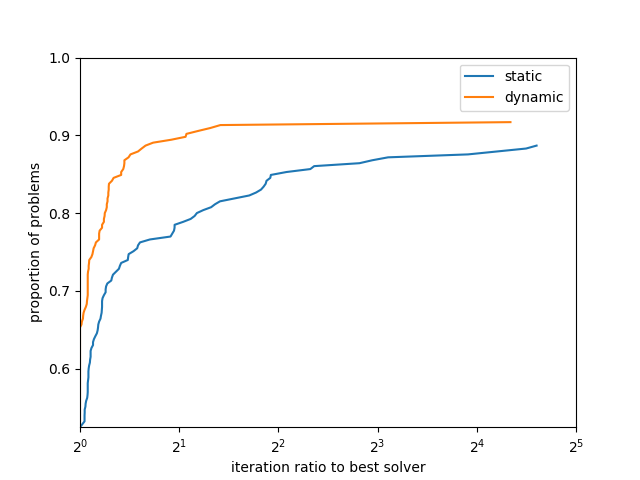
\includegraphics[scale=0.5]{ratios-dynamic-static.png}
%\caption{Comparison of dynamic and static $\mu$ updates for the one phase algorithm.}
%\end{figure}

In Figure~\ref{fig:ls-options} we trial different line search conditions for the stabilization steps. In particular, we compare the default setting of a `filter' as described in line~\eqref{line:sbl-backtrack} part (iii) of Algorithm~\ref{alg:stable} against other possible conditions. The first baseline to replace condition (iii) with  \eqref{phi-sufficient-progress} i.e. check that sufficient progress is made on the `log barrier' merit function. The other baseline is removing condition (iii) entirely and simple taking the maximum step possible. Figure~\ref{fig:ls-options} indicates that the filter has superior performance of these three options.

\begin{figure}[H]
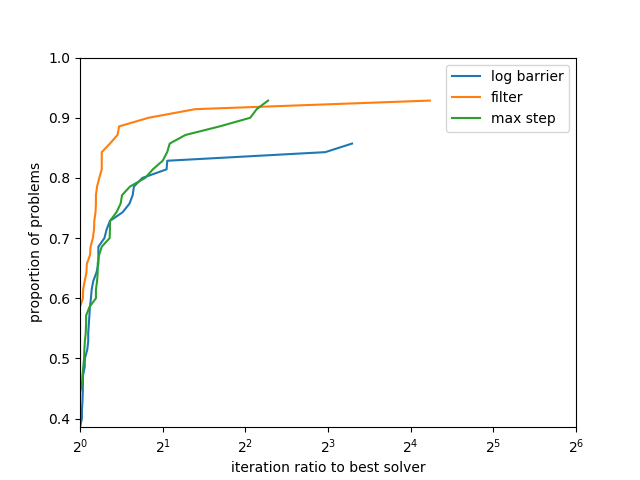
\includegraphics[scale=0.5]{ls-options.png}
\caption{Comparison of different line search options.}\label{fig:ls-options}
\end{figure}

In Figure~\ref{fig:num-corrections} we compare different choices of the parameter $c_{\max}$, the maximum number of corrections ($c_{\max}$ is used on line~\ref{take-steps} in Algorithm~\ref{one-phase-IPM}). As one would expect, increasing the number of corrections decreases the iteration count, but has little impact on the failure rate. In the actual implementation of our one phase algorithm we chose $c_{\max}=3$.
%can see the number of iterations is

\begin{figure}[H]
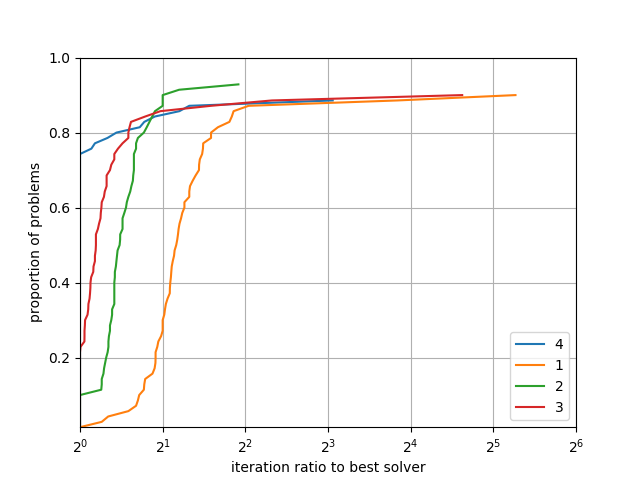
\includegraphics[scale=0.5]{num-corrections.png}
\caption{Comparison of the maximum number of corrections for the one phase algorithm.}\label{fig:num-corrections}
\end{figure}

\subsection{Comparison with IPOPT}\label{alg:comparison-IPOPT}

Please take these results with a grain of salt since we are comparing iteration counts not runtimes.

\todo[inline]{Comparison on number of function/constraint evaluations (clearly admit algorithm is not optimized to minimize constraint violation/function evaluation)}


We consider the final function values $f^{a}_{*}$ and $f^{b}_{*}$ of algorithm $a$ and $b$ respectively approximately the same if:
$$
\frac{f^{a}_{*} - f^{b}_{*}}{1 + \max \{ | f^{a}_{*} |, | f^{b}_{*} | \} } < 10^{-1},
$$
otherwise, we consider the solution of algorithm $a$ better than algorithm $b$ if $f^{a}_{*}  < f^{b}_{*}$. For problems where both algorithm find a KKT point this is reported in the top three rows of Table~\ref{tbl:pairwise-outcomes}. The remainder of Table~\ref{tbl:pairwise-outcomes} shows the number of times both algorithms succeed, fail, or just one algorithm fails. We consider the algorithm to have succeeded if it produces either a certificate of first order local optimality, infeasibility or unboundedness. 

Let us highlight a few interesting facts from the tables. The one phase algorithm seem to find better KKT points on $13$ problems versus $2$ for IPOPT (Table~\ref{tbl:pairwise-outcomes}). Furthermore, IPOPT fails on $39$ problems compared with $21$ problems for the one phase algorithm (Table~\ref{tbl:termination-status-counts}). A large proportion of these failures occur before IPOPT has started (Table~\ref{tbl:failure-reasons}).

\begin{table}[H]
\caption{Pairwise comparison of outcomes for IPOPT and the one phase algorithm}\label{tbl:pairwise-outcomes}
\begin{tabular}{ c c r }
  One Phase &  IPOPT &  \# \\
  \hline
same KKT & - & 158  \\
- & better KKT & 2 \\
better KKT & - &  13 \\
\hline
Succeed & Succeed & 185 \\
Fails & Fails & 7 \\
Succeed & Fails &  32 \\
Fails & Succeed & 14 \\
\end{tabular}
\end{table}

%Table~\ref{tbl:termination-status-counts} displays the 

\begin{table}[H]
\caption{Termination status counts}\label{tbl:termination-status-counts}
\begin{tabular}{ c c c r }
 &  One Phase &  IPOPT &  \\
  \hline
KKT &  201 & 191 \\
unbounded & 4 & 0  \\
primal infeasible & 12 &  8 \\
fail & 21 & 39 \\
\end{tabular}
\end{table}

\begin{table}[H]
\caption{Failure reasons}\label{tbl:failure-reasons}
\begin{tabular}{ c c c r }
 &  One Phase & IPOPT \\
  \hline
max time & 10 & 9  \\
max iter &  3 & 3 \\
error before starting & 4 & 19 \\
error during algorithm & 4 & 8 \\
\hline
total & 21 & 39
\end{tabular}
\end{table}

Figure~\ref{fig:comparison-IPOPT-on-CUTEst} compares the iterations that IPOPT and the one phase algorithm take to succeed (produce a certificate of first order local optimality, infeasibility or unboundedness) on the CUTEst test set. Note that the iteration counts for the solvers are similar, except that the one phase solver fails less frequently.


\begin{figure}[H]
\includegraphics[scale=0.5]{ratios-IPOPT-one-phase.pdf}
\includegraphics[scale=0.5]{iterations-IPOPT-one-phase.pdf}
%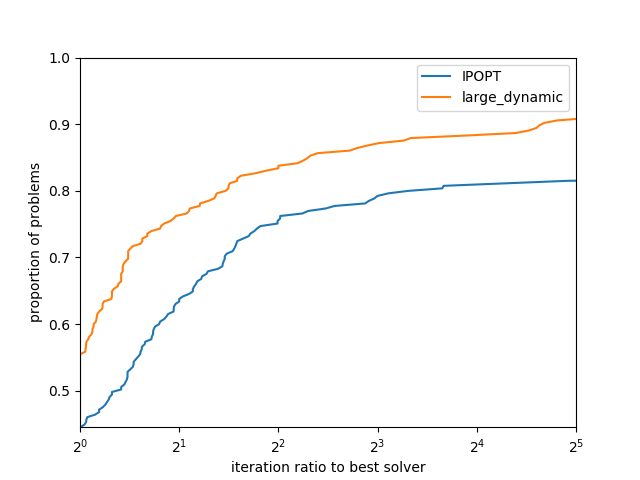
\includegraphics[scale=0.5]{ratios-n=50-10000.png}
%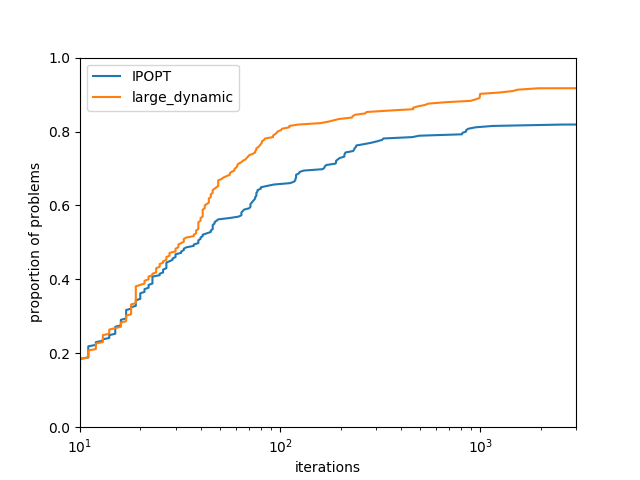
\includegraphics[scale=0.5]{iterations-n=50-10000.png}
\caption{Comparison of IPOPT and one phase on CUTEst for problems where at least one solver declared the problem optimal, infeasible or unbounded.}\label{fig:comparison-IPOPT-on-CUTEst}
\end{figure}

\todo[inline]{table or plot of maximum dual variables?}

\subsection{Comparison on infeasible problems}\label{sec:infeas}

Most of the CUTEst problems have feasible solutions. To generate a test set that was more likely to contain infeasible problems we perturbed the constraints as follows:
$$
\tilde{a}(x) = a(x) + e
$$
The solver terminated with the statuses described in the Table~\ref{tbl:termination-status-counts-peturbed}. This test was only run on problems with at most $1,000$ variables and constraints total.
\begin{table}[H]
\caption{Termination status counts for perturbed CUTEst problems.}\label{tbl:termination-status-counts-peturbed}
\begin{tabular}{ c c c r }
 &  One Phase &  IPOPT &  \\
  \hline
KKT & 22 & 20 \\
unbounded & 1 & 0  \\
primal infeasible & 44 &  38 \\
fail & 3 & 12 \\
\end{tabular}
\end{table}

Next, in Figure~\ref{fig:comparison-IPOPT-on-perturbed-CUTEst} we compare IPOPT and the one phase on the subset problems which at least one solver declared the problem locally infeasible. From this figure one can see that the one phase solver is quicker and more robust than IPOPT.

\begin{figure}[H]
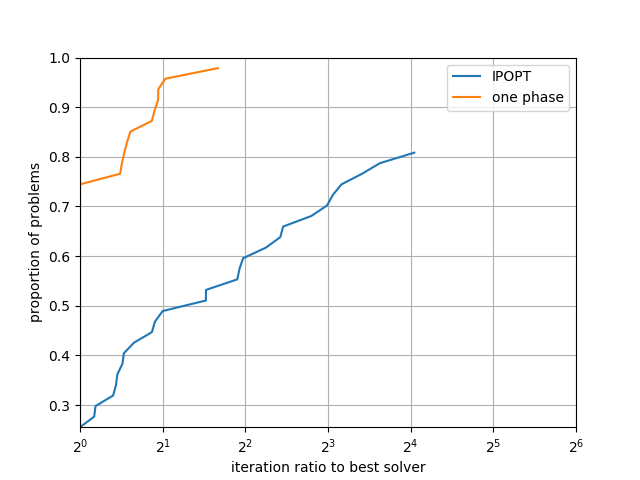
\includegraphics[scale=0.5]{infeas-ratios.png}
\caption{Comparison of IPOPT and one phase on perturbed CUTEst problems for which at least one solver declares the problem locally infeasible.}\label{fig:comparison-IPOPT-on-perturbed-CUTEst}
\end{figure}

%
%\subsection{Comparison on NETLIB for linear programming}\label{sec:netlib}
%
%The purpose of this Section is to show that the one phase algorithm has good performance on linear programs, as one would expect since the algorithm is heavily influenced by ideas from linear programming [REF]. My experience from our previous paper is that there is a huge difference in the performance of IPOPT and the one phase algorithm.
%
%[Use IPOPT option specialized for LP]
%
%\begin{figure}[H]
%\missingfigure{...}
%%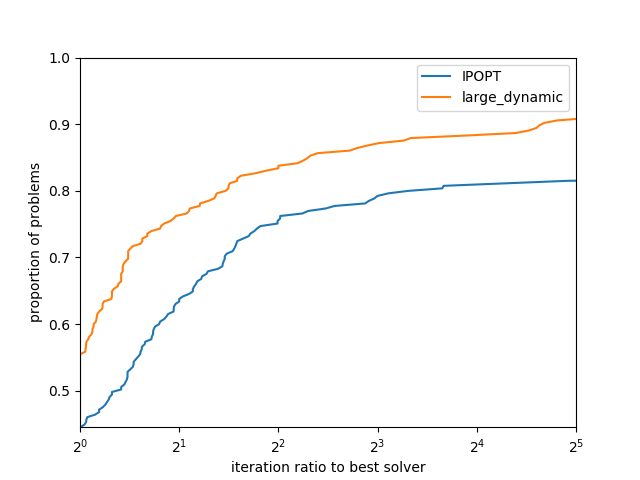
\includegraphics[scale=0.5]{ratios-n=50-10000.png}
%%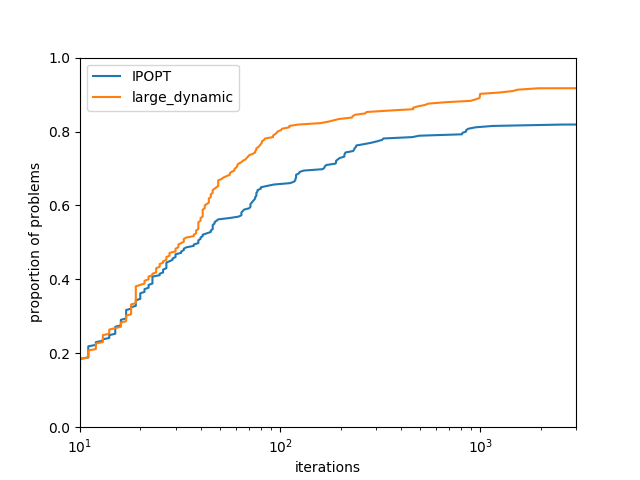
\includegraphics[scale=0.5]{iterations-n=50-10000.png}
%\caption{Comparison of IPOPT and one phase on the NETLIB linear programming test set.}
%\end{figure}


\section{Conclusions}
\begin{enumerate}
\item ??
\end{enumerate}


\section{To do}

\begin{enumerate}
\item clean up 
\item edit code to match document
\item run full CUTEst test
\end{enumerate}

\bibliographystyle{apalike}
\bibliography{library-one-phase-2.bib}


\appendix

\section{Matrix factorization strategy}

This strategy is based on the ideas of IPOPT \cite[Algorithm IC]{wachter2006implementation}.

\begin{algorithm}[H]
\textbf{Input:} The matrix $\mathcal{K}_{0}$ and current delta choice $\delta$ \\
\textbf{Output:} The factorization $\mathcal{K}_{\delta}^{-1}$ for some $\delta > 0$ such that the matrix $\mathcal{K}_{\delta}$ has the correct inertia.
\begin{enumerate}[label*=A.{\arabic*}]
\item Set $\delta_{\text{prev}} \gets \delta$
\item Set $\delta \gets 0$
\item Perform LDL factorization of $\mathcal{K}_{\delta}$, if inertia is correct return $\mathcal{K}_{\delta}^{-1}$ otherwise continue.
\item If $\delta_{prev} > 0$ set $\delta \gets \max\{ \parDeltaMin, \delta_{\text{prev}} / 3 \}$ otherwise set $\delta = \delta_{\text{start}} \mu$.
\item Perform LDL factorization of $\mathcal{K}_{\delta}$, if inertia is correct return $\mathcal{K}_{\delta}^{-1}$ otherwise continue.
\item Set $\delta \gets 8 \delta$. Go to previous step.
\end{enumerate}
\caption{Matrix factorization strategy}\label{alg:mat-fact}
\end{algorithm}

\section{The (non-existence) of a central path in non-convex optimization}\label{app:non-existence-of-central-path}

Would be nice to have a long discussion on this issue

$$
f_{\mu}(x) = 50 (x - 0.5)^3 + x - \mu (\log(x) + \log(1 - x))
$$

$$
\nabla f_{\mu}(x) = 150.0 * (x - 0.5)^2 + 1.0  - \mu / x + \mu / (1 - x) = 0 \\
$$
Is discontinuous at $\mu = 3$, $x \approx 0.5$ i.e. there exists no function $x(\mu)$ such that $\nabla f_{\mu}(x(\mu)) = 0$ and $x(\mu)$ is continuous. 

[Vanderbei' s example for the problem $\min{ x -x^2}$ s.t. $x \ge 0$ there exists no continuous central path from an initial point to the optimal solution. However, optimal solution is unbounded.]


\section{Old}

\subsection{Intuition: penalty method versus infeasible start method}

Give a simple example illustrating the draw backs of a penalty method
\begin{enumerate}
\item Makes the algorithm more complex
\item If penalty parameter is too big then problem is harder to solve than it should be
\item When penalty parameter is updated the dual feasibility increases suddenly
\end{enumerate}

\subsection{Discussion of Watcher and Biegler's example}

Key differences:
\begin{enumerate}
\item Non-linear updates
\item Initialization of slack variables violates their assumptions
\end{enumerate}

\begin{flalign}
x_{1}^2 + a \ge 0 \\
x_{1} \ge b
\end{flalign}

\begin{flalign}
\min{ -\vioVar (x_{1}^2 + a) - (x_{1} - b) } \\
w \ge 0
\end{flalign}
At 
$$
\vioVar = 1 / (2 x_{1})
$$



\subsection{Relevant literature}

Within non-convex optimization there are four papers that I think are particularly relevant to our work:

\begin{enumerate}
\item The paper \cite{wachter2000failure} shows that there are examples for which infeasible start algorithms will always fail to converge to either a optimal solution or a stationary measure of infeasibility when constraints are non-convex (irrespective of the strategy for used). This is the inspiration for the two phase algorithm of IPOPT and justifies why our one phase algorithm is necessary.
\item The description of the IPOPT algorithm \cite{wachter2005line}. IPOPT uses a two phase method the primary phase searches simultaneously for optimality and feasibility using a classical infeasible start method and a feasibility restoration phase that minimizes infeasibility. The feasibility restoration phase is only called when the step size for the infeasible start method is small. Another distinct feature of the algorithm is the filter line search (which allows progress on either the constraints or the objective).
\item The description of the KNITRO algorithm \cite{byrd2006knitro}. KNITRO is a trust region algorithm. The approach is quite distinct from typical infeasible start algorithms and is worth looking at (each step computes two different directions, using two different linear systems, one to reduce the objective and the other to reduce infeasibility). There is a more recent paper \cite{nocedal2014interior} that adds an feasibility restoration phase (this is theoretically unnecessary, but the practical results are good). 
\item The paper \cite{curtis2012penalty} introduces a barrier penalty method. This paper uses a similar approach to us. The main different with our approach is we treat $\lambda$ as a dual variable, whereas in Curtis's paper $\lambda$ is replaced by a penalty parameter that is updated in an ad hoc fashion.
\item Papers in convex optimization?
\item why homogenous algorithm fails: relies on KKT conditions to measure progress
\end{enumerate}



\subsection{Old convergence proofs}


I keep on re-writing these as the algorithm changes, so the current proofs are not up to date. Will revise these once the algorithm stabilizes.

\newcommand{\algBlurb}{Consider Algorithm~\ref{one-phase-IPM}.
Assume that the slack variables are initialized such that $s^{1} \gets \vioVar^{1} \conWeight - a(x^{1})$ for some $\vioVar^{1}, \conWeight \ge 0$ such that $s^{1} > 0$.}

\begin{lemma}
\algBlurb{}
If the criterion for an aggressive step \eqref{agg-criteron} is met at any point during the algorithm then for the current dual variable $y$ we have:
$$
\| y^k \|_{1} \le \frac{\| \nabla f(x^{k}) \|_{2}}{\TOLinf^2} + 3 m
$$

$$
\conWeight^T y^k \le \frac{ \| \nabla f(x^{k}) \|_{2} + \mu (1 + \| W \|_{\infty} )}{ \vioVar^k \TOLinf }
$$
%$$
%s^{k} \ge \frac{\mu \TOLopt^2}{\| \nabla c(x^{k}) \|_{2} + 1}
%$$
\end{lemma}

\begin{proof}
Observe that:
$$-a(x)^T y = -(a(x) - s)^T y - s^T y \ge  \mu (e^T y - 2)$$
Therefore:
$$
\frac{\| \nabla a(x)^T y \|}{-a(x)^T y} \le \frac{\mu^k \sqrt{ \| y \|_{1} + 1} + \| \nabla c(x) \|}{\mu ( \| y \|_{1} - 2 m )} 
$$
If:
$$
\| y^k \|_{1} \ge \frac{\| \nabla c(x^{k}) \|_{2} +  3 m}{\TOLopt^2} 
$$
Then:
$$
\frac{\| \nabla a(x)^T y \|}{-a(x)^T y} \le \epsilon 
$$
Which gives the result.
\end{proof}

\begin{proof}
Observe that:
$$-a(x)^T y = -(a(x) - s)^T y - s^T y \ge  \mu (e^T y - 2)$$
Therefore:
$$
\frac{\| \nabla a(x)^T y \|}{-a(x)^T y} \le \frac{1+ \| \nabla c(x) \|}{\mu ( \| y \|_{1} - 2 m )} 
$$
If:
$$
\| y^k \|_{1} \ge \frac{\| \nabla c(x^{k}) \|_{2}}{\TOLopt^2} +  3 m
$$
Then:
$$
\frac{\| \nabla a(x)^T y \|}{-a(x)^T y} \le \epsilon 
$$
Which gives the result.
\end{proof}

\begin{lemma}
\algBlurb{}
Algorithm~\ref{one-phase-IPM} takes at most $\frac{\mu^{0} (2 \| \nabla c(x^{k}) \|_{2} + 8)}{\epsilon^2}$ aggressive steps to satisfy the termination criterion i.e satisfy \termination{}.
\end{lemma}

\begin{proof}
We wish to prove that for any $\delta$ with
$$
\delta \ge \frac{\| g^k \| L_0}{\mu^k} - \lambda_{\min}{(M^{k})}
$$
and $\alpha$ satisfying
\begin{flalign}\label{assume-alpha}
\alpha \le \frac{1}{\| y^k \|_{\infty} + 4} %\frac{\min_{i}\{s^{k}_{i}\}}{4 \mu^k}
\end{flalign}
the iterate $x^{+} = x^{k} + \alpha d_{x}^k$, $y^{+} = y^{k} + \alpha d_{y}^k$, $\mu^{+} = \mu (1 - \alpha )$ is feasible. Observe that this implies the result since if:
$\alpha \ge \frac{1}{2 (\| y^k \|_{\infty} + 4)}$ %\frac{\min_{i}\{s^{k}_{i}\}}{4 \mu^k}
then:
 $$
 \mu^{k+1} = (1 - \alpha) \mu^{k} = \mu^k - \frac{\mu^k}{2 \| y^k \|_{\infty} + 8} \le \mu^k - \frac{\epsilon^2}{2 \| \nabla c(x^{k}) \|_{2} + 8}.
  $$
We wish to show that $ s^{k+1}  \in [s^k / 2, 3 s^{k} / 2]$. Where $s^{k+1} = a(x + \alpha_{P} d_{x}) + (1 - \alpha_{P} ) \mu^k e$. Subtracting and adding $s^k = a(x^k) + \mu^k e$ yields
$$
s^{k+1} = s^k + ( a(x^k + \alpha_{P}^k d_{x}^k ) - a(x^k)) - \alpha_{P}^k \mu^k e
$$
Therefore, it remains to bound the term $a(x^{k} + \alpha_{P}^k d_{x}^{k}) - a(x^k)  - \alpha_{P}^k \mu^k e$. Applying our assumption on $\alpha^{k}$, we immediately get $0 \le \alpha_P^{k} \mu^k e \le  s^{k} / 4$. Furthermore, we know that 
$\| d_{x}^{k} \|_{2} \le \mu^k L_0$ therefore:
$$
\alpha_{P}^{k} \| d_{x}^{k} \|_{2} \le \frac{\min_{i}\{ s^{k}_{i} \}}{2 L_{0}}
$$
Since $a(x)$ is $L_{0}$-Lipshitz we have:
$$
-s^k / 4 \le a(x^k) - a(x^{k} + \alpha_{P}^{k} d_{x}^{k})  \le s^k / 4
$$
which shows that $s^{k+1} \in [s^k/2, 2 s^k]$. Observe that $y^{k+1} = y^{k} + \alpha^k d_{y}^k \ge y^k / 2$. It remains to show that $\| y^{k+1} s^{k+1} - \mu^{k+1} \|_{\infty} \le \mu^k / 2$. Now we have:
$$
d_{y}  = - Y (S^{-1} d_{s} + e)
$$
Hence using that $\| d_{s} \| \le ...$ we get $d_{y} \in [-2y, 2y]$. It follows that $y^k + \alpha_{P} d_{y} \in [ y^{k} / 2, 3 y^{k} / 2]$. 

Finally, using the fact that $s^{k+1}  \in s^{k} [3/4, 5/4]$ and $s^{k+1} \in y^{k} [3/4, 5/4]$  we have: 
$$
\frac{s^{k+1} y^{k+1}}{s^k y^k} \in [1/2, 3/2]
$$
And since $\frac{s^{k} y^{k}}{\mu^k} \in [1/2,3/2]$ we have  $\frac{s^{k+1} y^{k+1}}{\mu^k} \in [1/4,3]$ which concludes the proof.
\end{proof}



\end{document}